\chapter{Desenvolvemento do sistema}
\minitoc
\label{chap:implementacion}
\vspace{0.5cm}

%%%%%%%%%%%%%%%%%%%%%%%%%%%%%%%%%%%%%%%%%%%%%%%%%%%%%%%%%%%%%%%%%%%%%%%%%%%%%%%%
% Objetivo: Exponer las partes relevantes de la implementación                 %
%%%%%%%%%%%%%%%%%%%%%%%%%%%%%%%%%%%%%%%%%%%%%%%%%%%%%%%%%%%%%%%%%%%%%%%%%%%%%%%%

\lettrine{N}{este} capítulo exporase o desenvolvemento do proxecto baseándose
no esquema proporcionado pola planificación inicial: desde o deseño software e
hardware de baixo nivel do sistema ata a implementación e o ensamblado do
producto, pasando por un prototipo operacional.

\section{Determinación}

 \subsection{Obxectivos}

 Establecéronse os obxectivos da fase de desenvolvemento do proxecto. \\

 Obxectivos:

 \begin{itemize}
  \item Implementar unha gaita MIDI sen fíos en tempo real empregando
        software/hardware libre.
 \end{itemize}

 \subsection{Alternativas}

 Establecéronse posibles alternativas a eses obxectivos, aplicables no caso de
 que estes non se puidesen cumprir. \\

 Alternativas:

 \begin{itemize}
  \item Se non é posible implementar completamente o proxecto, pode optarse
        por:
        \begin{enumerate}
         \item Se é por causa de que o hardware non o permite, cambiar as pezas
               correspondentes por outras que si o permitan.
         \item Se as partes que non é posible implementar son opcionais ou de
               pouco peso, desbotalas e implementar o resto.
         \item Cancelar e mudar de proxecto.
        \end{enumerate}
 \end{itemize}

 \subsection{Restriccións}

 Establecéronse restriccións aplicables a ditos obxectivos.

 \begin{enumerate}
  \item As propias restriccións veñen dadas polo propio título do proxecto. A
        saber:
        \begin{enumerate}
         \item Empregar o protocolo MIDI.
         \item Empregar tecnoloxía sen fíos.
         \item Empregar tempo real.
         \item Empregar software libre.
         \item Empregar harwdware libre.
         \item E/ou as derivadas de calquera das súas alternativas.
        \end{enumerate}
 \end{enumerate}

\section{Avaliación de alternativas e resolución de riscos}

 \subsection{Análise de riscos}

 Determináronse os riscos que comportaban as distintas alternativas e as súas
 posibles solucións.

 \begin{enumerate}
  \item Alternativas 1.
        \begin{enumerate}
         \item Riscos:
               \begin{enumerate}
                \item Que non exista hardware alternativo que soporte a
                      implemtación das características restantes.
                \item Que as partes a desbotar sexan partes importantes ou
                      incluso críticas.
                \item Que o tempo restante para a execución do proxecto non
                      sexa suficiente.
               \end{enumerate}
         \item Solucións:
               \begin{enumerate}
                \item Recortar características ou cancelar e mudar de proxecto.
                \item Aplicar medidas de mitigación para que a planificación
                      non se vexa afectada en extremo, ou cancelar e mudar de
                      proxecto se fan inviable o mesmo.
                \item Agardar a presentalo na seguinte convocatoria.
               \end{enumerate}
        \end{enumerate}
 \end{enumerate}

 \subsection{Prototipo operacional}
 
 Nesta fase desenvolveuse o seguinte nivel de prototipado, tanto hardware coma
 software, sendo xa ambos operacionais. \\
 
 A aproximación seguida foi aplicar \textit{BDD} \cite{BDD} ou \textit{TDD}
 \cite{TDD} segundo o caso, en dirección \textit{top-dowm} obtendo así as
 sinaturas dos servizos e o comportamento desexado dos mesmos primeiro, para
 logo facer unha implementación \textit{bottom-up} respectando o deseño
 conseguido previamente.

  \subsubsection{Prototipo hardware}
  
  Para a o prototipo hardware operacional tiramos do prototipo deseñado na fase
  anterior, para o cal empregamos ferramentas CAD co fin de poder facer probas
  en formato dixital antes de pasar a formato físico, evitando así os múltiples
  problemas relacionados.

   \paragraph{Integración do hardware}
   
   Unha vez claro o deseño sobre o papel, montouse un prototipo físico con cada
   compoñente por separado, de maneira que inicialmente se puidera probar cada
   un de maneira unitaria, antes de pasar á integración final. \\
   
   Desta maneira, dividiuse a montaxe completa en varias submontaxes:
   
   \begin{itemize}
    \item Router (figura \ref{figura:Router}).
    \item Receptor (figura \ref{figura:Receptor}).
    \item Sensor de presión (figura \ref{figura:SensorPresion}).
    \item Sensores capacitivos (figura \ref{figura:SensoresCapacitivos}).
    \item Lector de tarxetas (figura \ref{figura:LectorTarxetas}).
   \end{itemize}
   
   A primeira montaxe foi a do router por resultar a máis sinxela, xa que
   consistiu nunha placa Arduino Uno sobre a que se montou unha placa auxiliar
   onde se montou o transmisor XBee, todo sen maior problema por ser altamente
   acoplables, sendo logo embebidos nunha caixa a medida e conectados por USB
   ó ordenador onde se executa a aplicación de configuración e o servidor
   MIDI. \\
   
   A nivel de sinatura de servizos, ó funcionar coma un simple router
   automatizado, non tiña máis que probar a transmisión correcta de datos, que
   decidiu deixarse coma último punto da integración hardware por razóns de
   fiabilidade na transmisión dos mesmos. \\
   
   \begin{figure}[htbp]
    \centering
    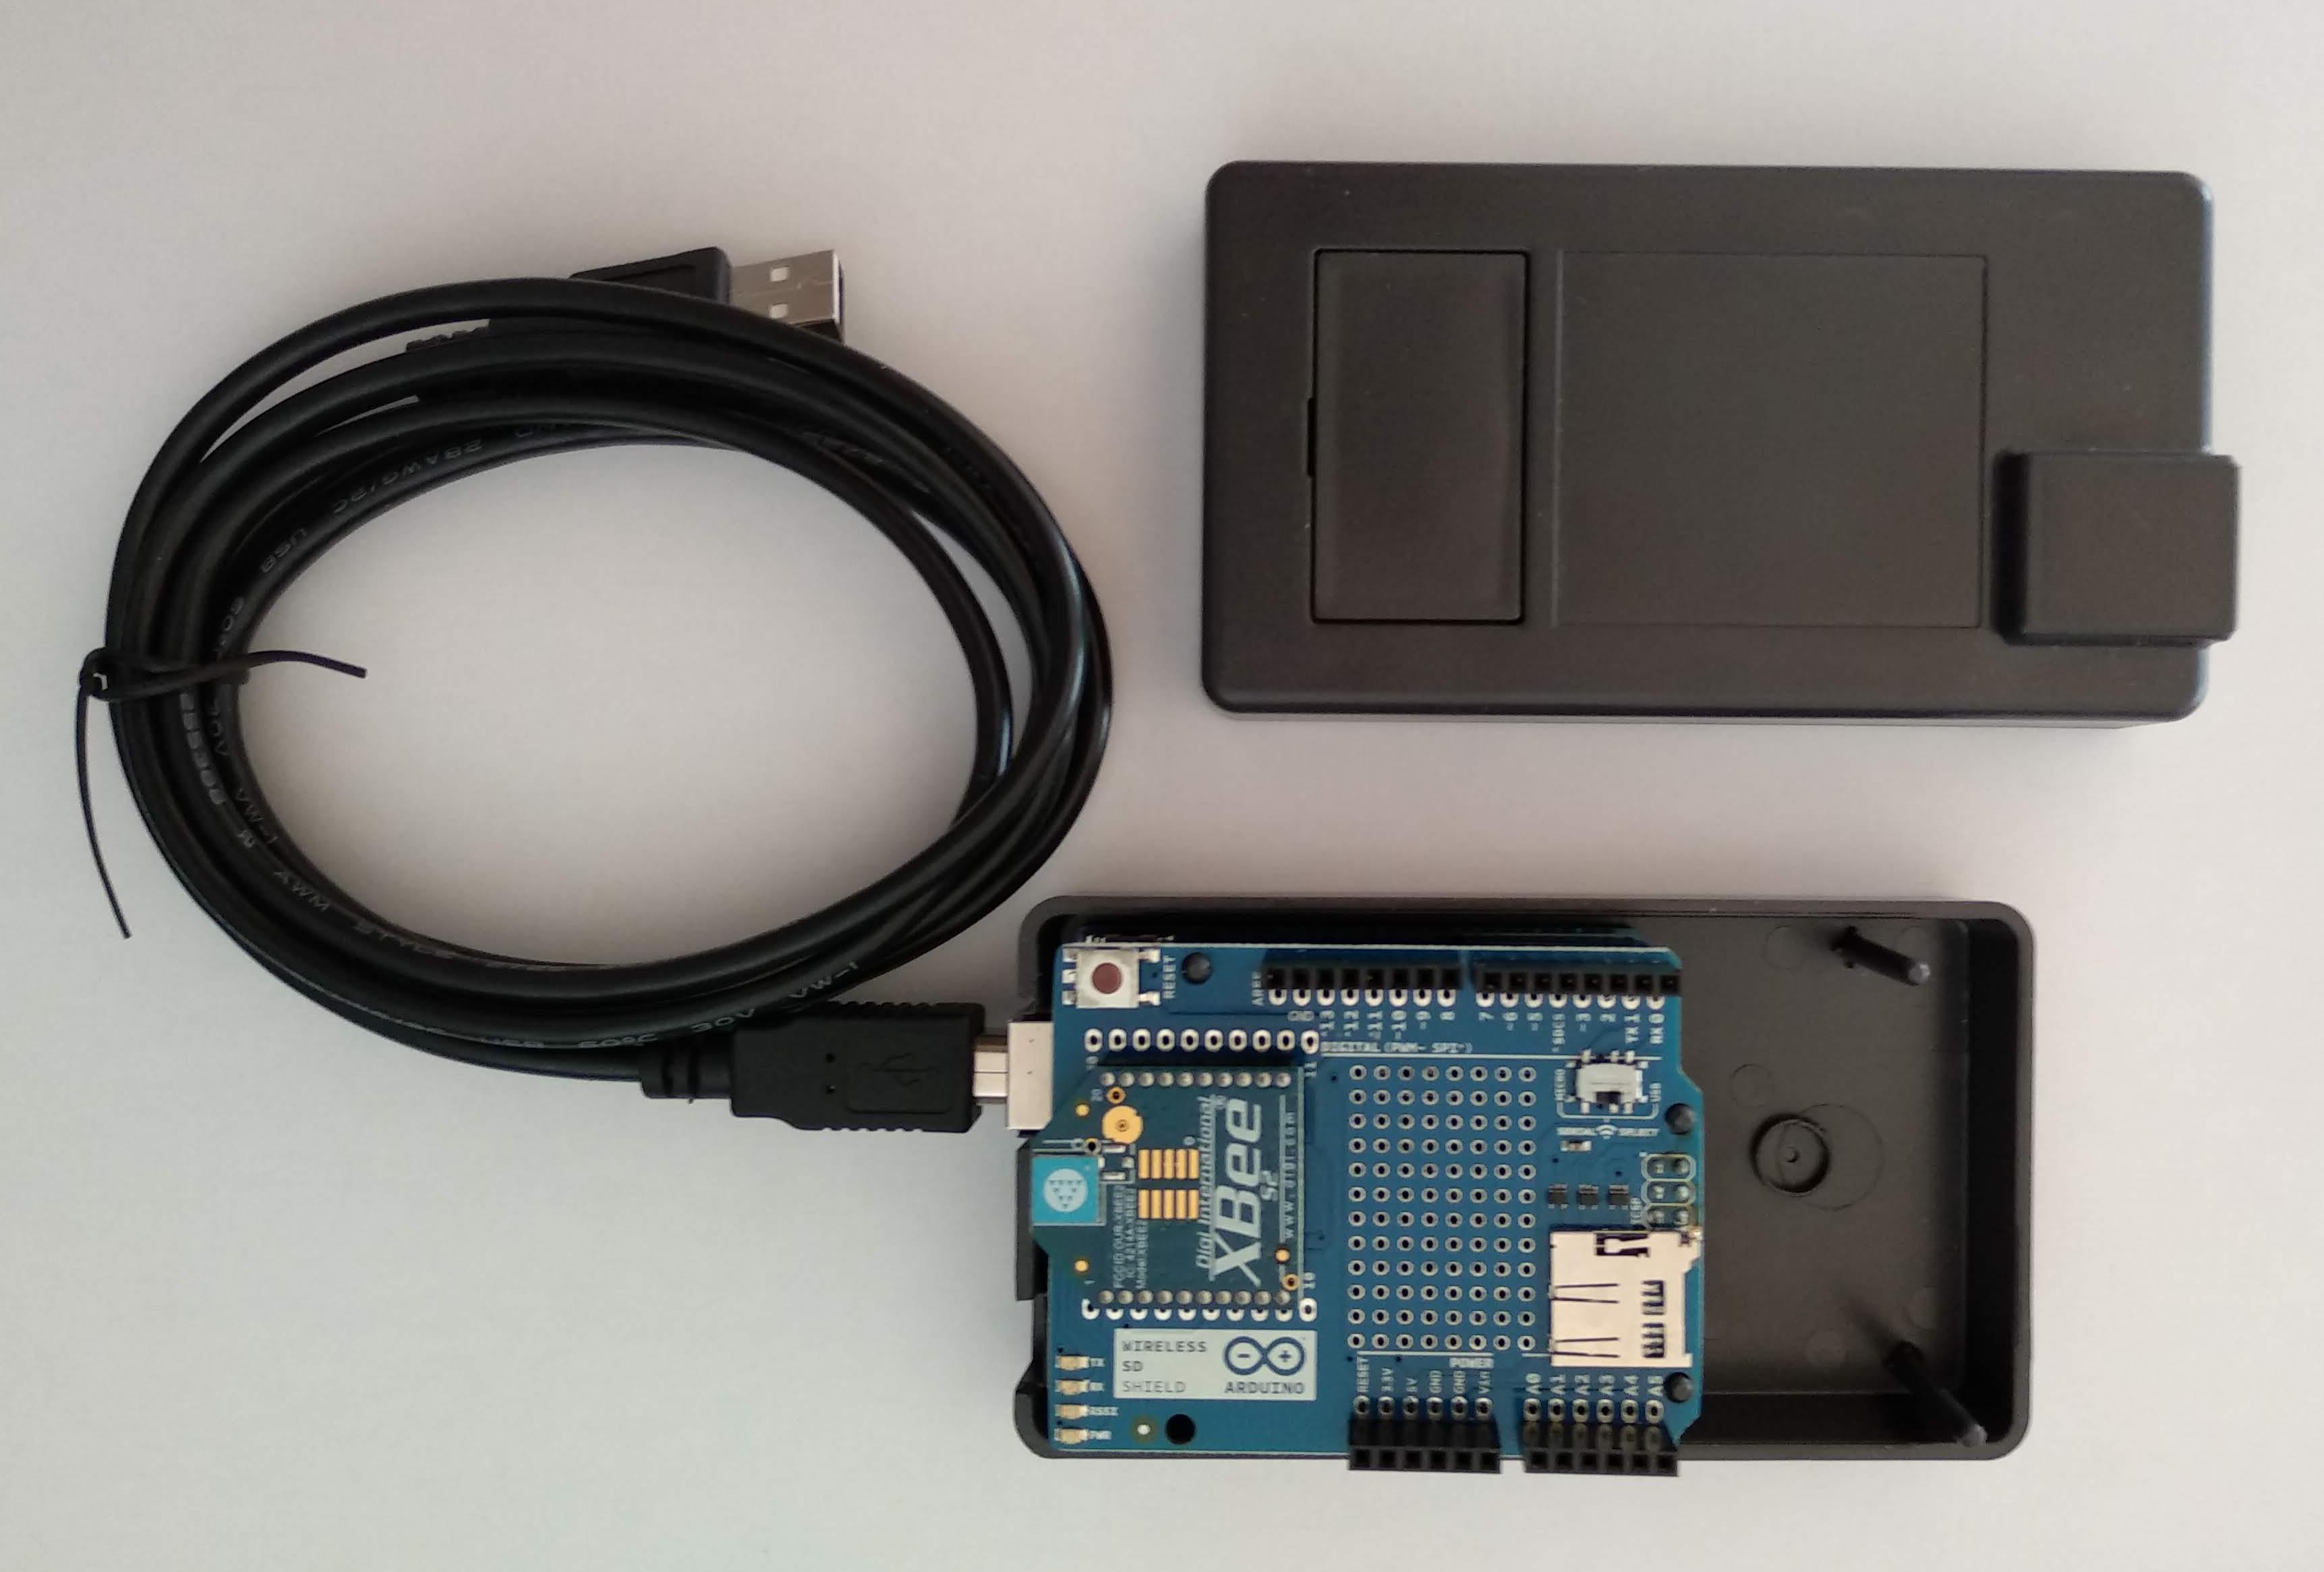
\includegraphics[scale=0.15,keepaspectratio=true]{./imagenes/router.jpg}
    % router.jpg: 640x480 pixel, 72dpi, 22.58x16.93 cm, bb=0 0 640 480
    \caption{Router}
    \label{figura:Router}
   \end{figure}
   
   A seguinte montaxe foi a do receptor, moi similar á do router, pois non deixa
   de ser unha placa Arduino Fio, que xa dispón dun zócalo para o módulo XBee e
   polo que non precisa de placa auxiliar. \\
   
   Polo mesmo motivo que o anterior, deixouse para máis adiante coma o último
   punto ou nivel de integración, pois resulta máis robusto probar e medir
   primeiro de maneira cableada e logo pasar ó modo sen fíos e poder comparar
   medicións e resultados. \\
  
   \begin{figure}[htbp]
    \centering
    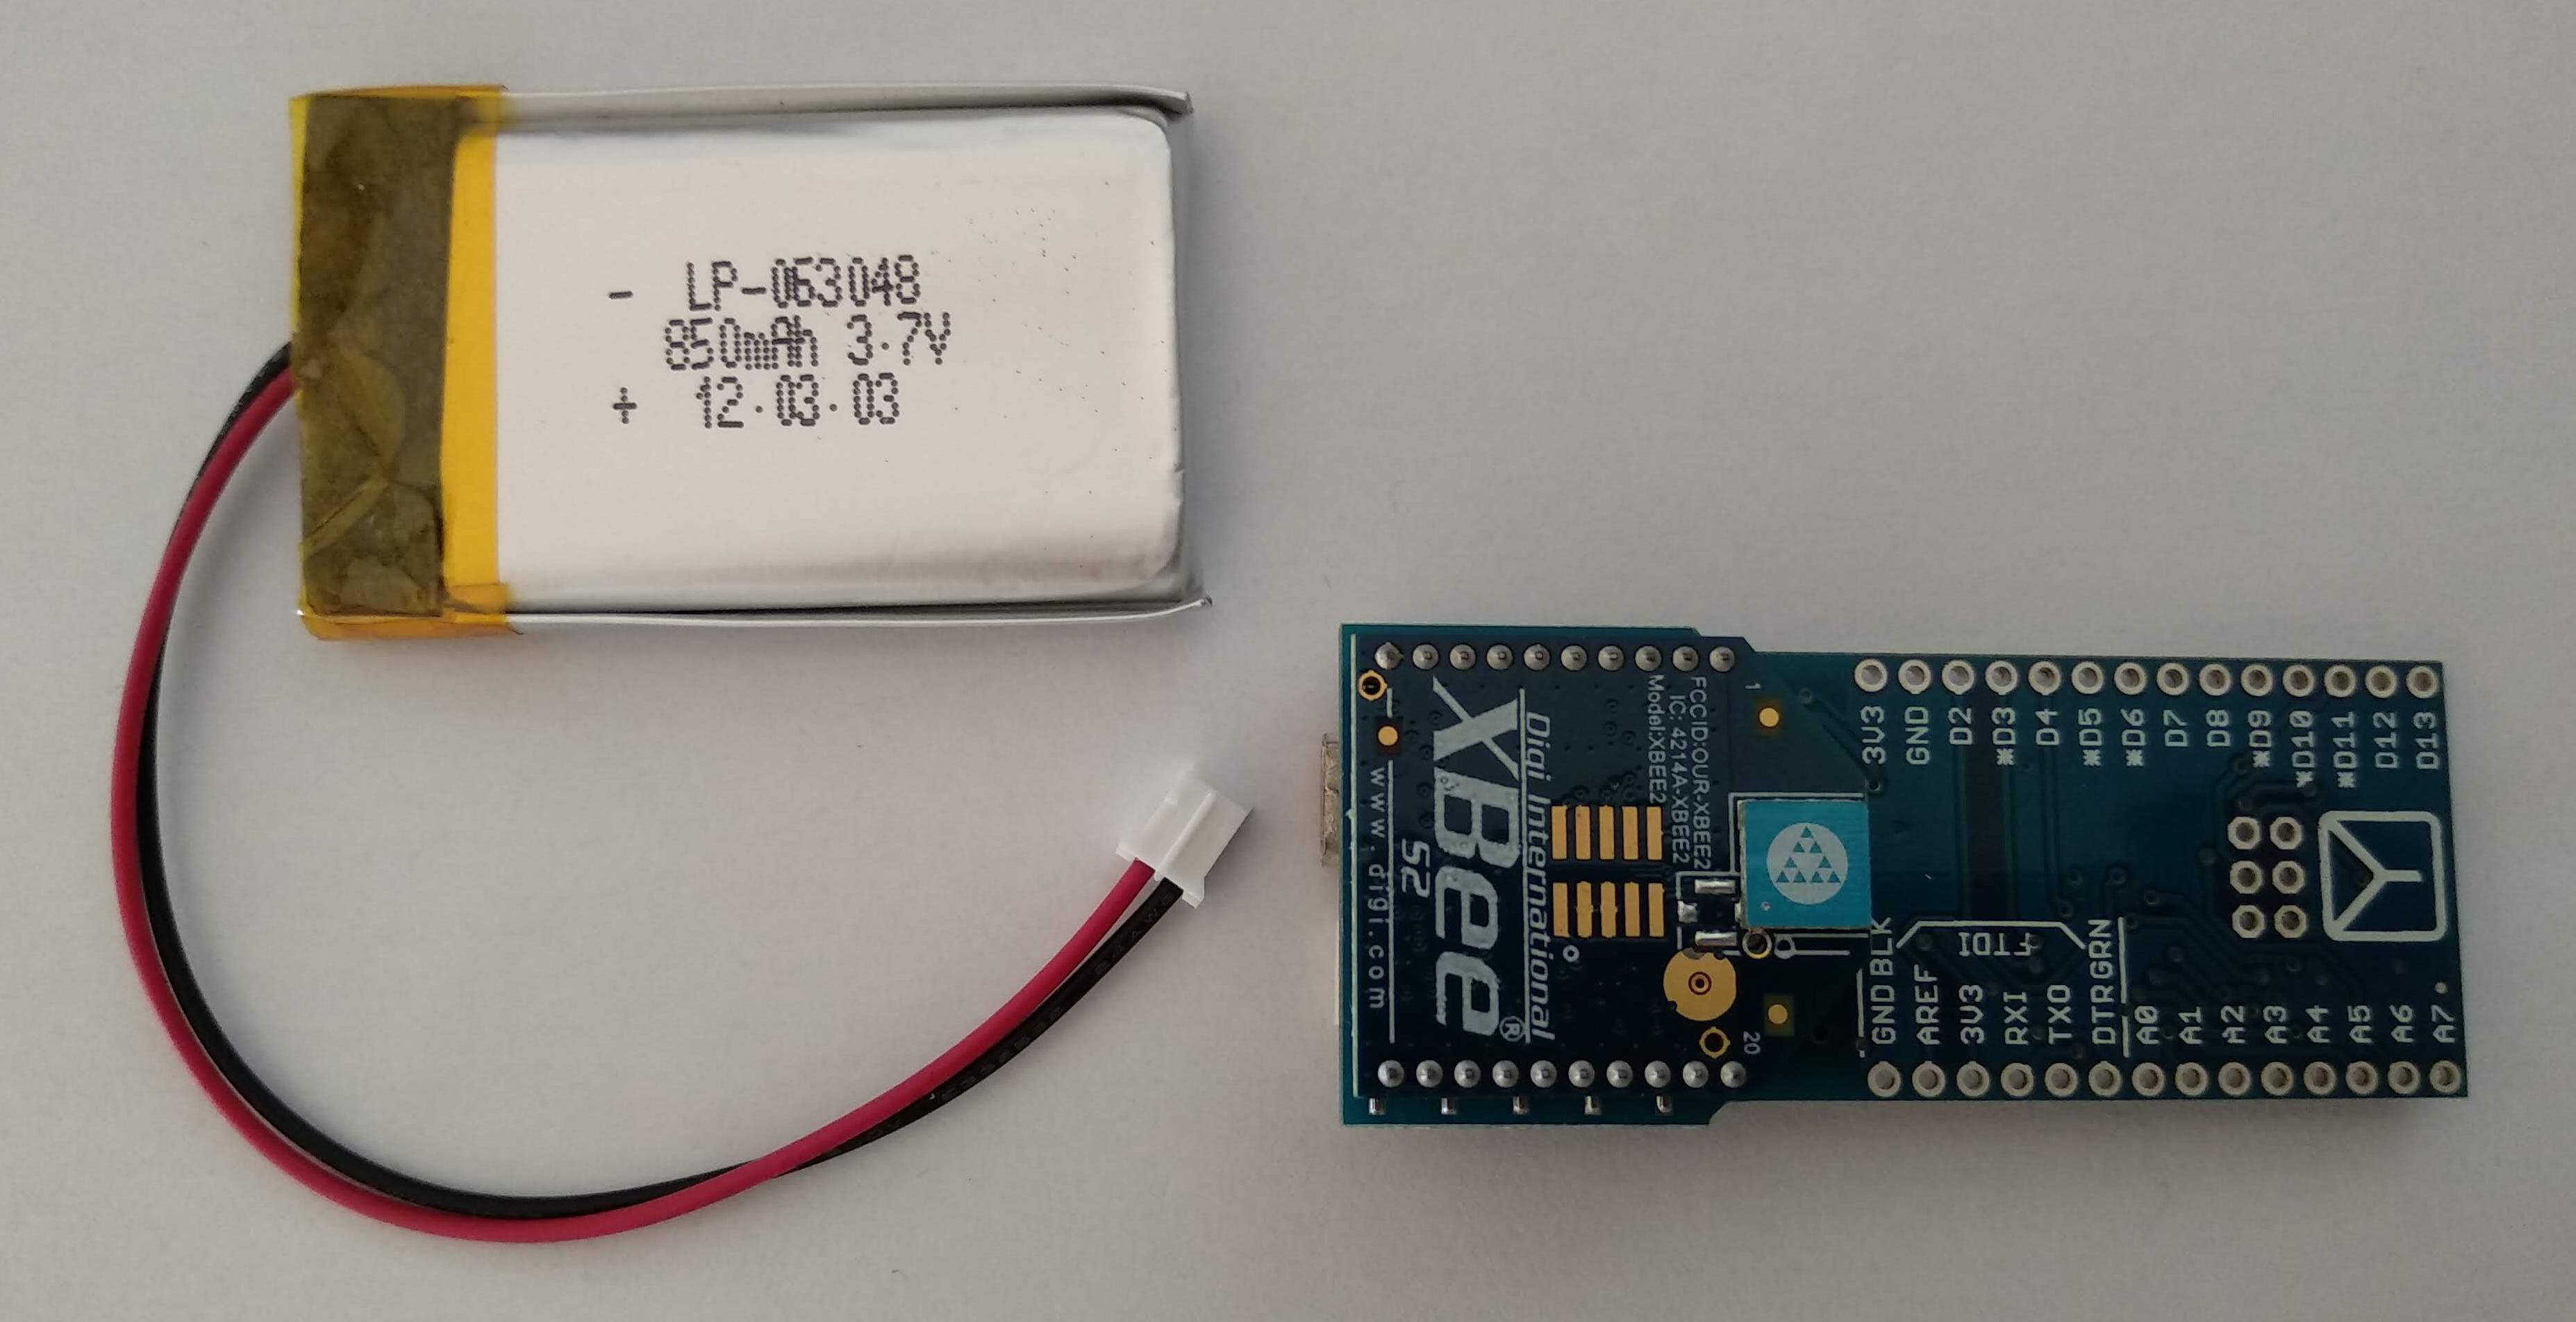
\includegraphics[scale=0.15,keepaspectratio=true]{./imagenes/receptor.jpg}
    % receptor.jpg: 640x480 pixel, 72dpi, 22.58x16.93 cm, bb=0 0 640 480
    \caption{Receptor}
    \label{figura:Receptor}
   \end{figure}
   
   No seu lugar, para desenvolver a lóxica de negocio da gaita MIDI, empregouse
   unha placa Arduino Uno, que conta coas mesmas características, salvo pola
   conexión directa do módulo XBee e que conta coa vantaxe de que podemos
   descargar nela o firmware da nosa implementación directamente a través dun
   cable USB. \\
   
   Neste caso a interface pública veu definida polo propio funcionamento de
   Arduino, contando cun método de configuración inicial e outro de execución
   continua. \\
   
   O que fixemos neste caso foi facer unha primeira implementación en
   pseudo-código do comportamento xeral que tería o dispositivo, intentando
   ver a qué periférico tería que chamar en cada caso, cándo e cómo, dando como
   resultado dúas partes claramente diferenciadas:
   
   \begin{itemize}
    \item Configuración das características propias da gaita.
    \item E reproducción ou envío de mensaxes MIDI.
   \end{itemize}
   
   Na parte de configuración, realizaríase tanto a carga dos parámetros
   configurables ó inicio coma o intercambio de configuracións entre o
   dispositivo e a aplicación de configuración, para o que sería preciso tirar
   do lector de tarxetas para persistir a información, así coma unha librería
   JSON para darlle formato un formato usable á mesma e da que falaremos máis
   adiante. \\
   
   En canto á parte de reproducción, sería preciso avaliar a presión do fol para
   decidir se o dispositivo debe soar ou non e a dixitación actual a través dos
   sensores capacitivos para ver se corresponde con algunha válida e por tanto
   producir o son relativo á mesma mediante o emprego dunha librería MIDI da que
   tamén falaremos máis adiante. \\
   
   Ampliaremos esta lóxica polo miúdo cando cheguemos á parte software, facendo
   uso de diagramas de fluxo. \\
   
   A continuación procedeuse co sensor de presión, por ser o seguinte máis
   sinxelo en orde de funcionalidade, pois o único que precisamos obter del é a
   presión dentro do fol, aínda que pode devolver máis parámetros relacionados
   coa mesma. \\
   
   Como se pode ver na imaxe, conectouse a unha placa Arduino Uno empregando
   o bus I2C do mesmo. \\
  
   \begin{figure}[htbp]
    \centering
    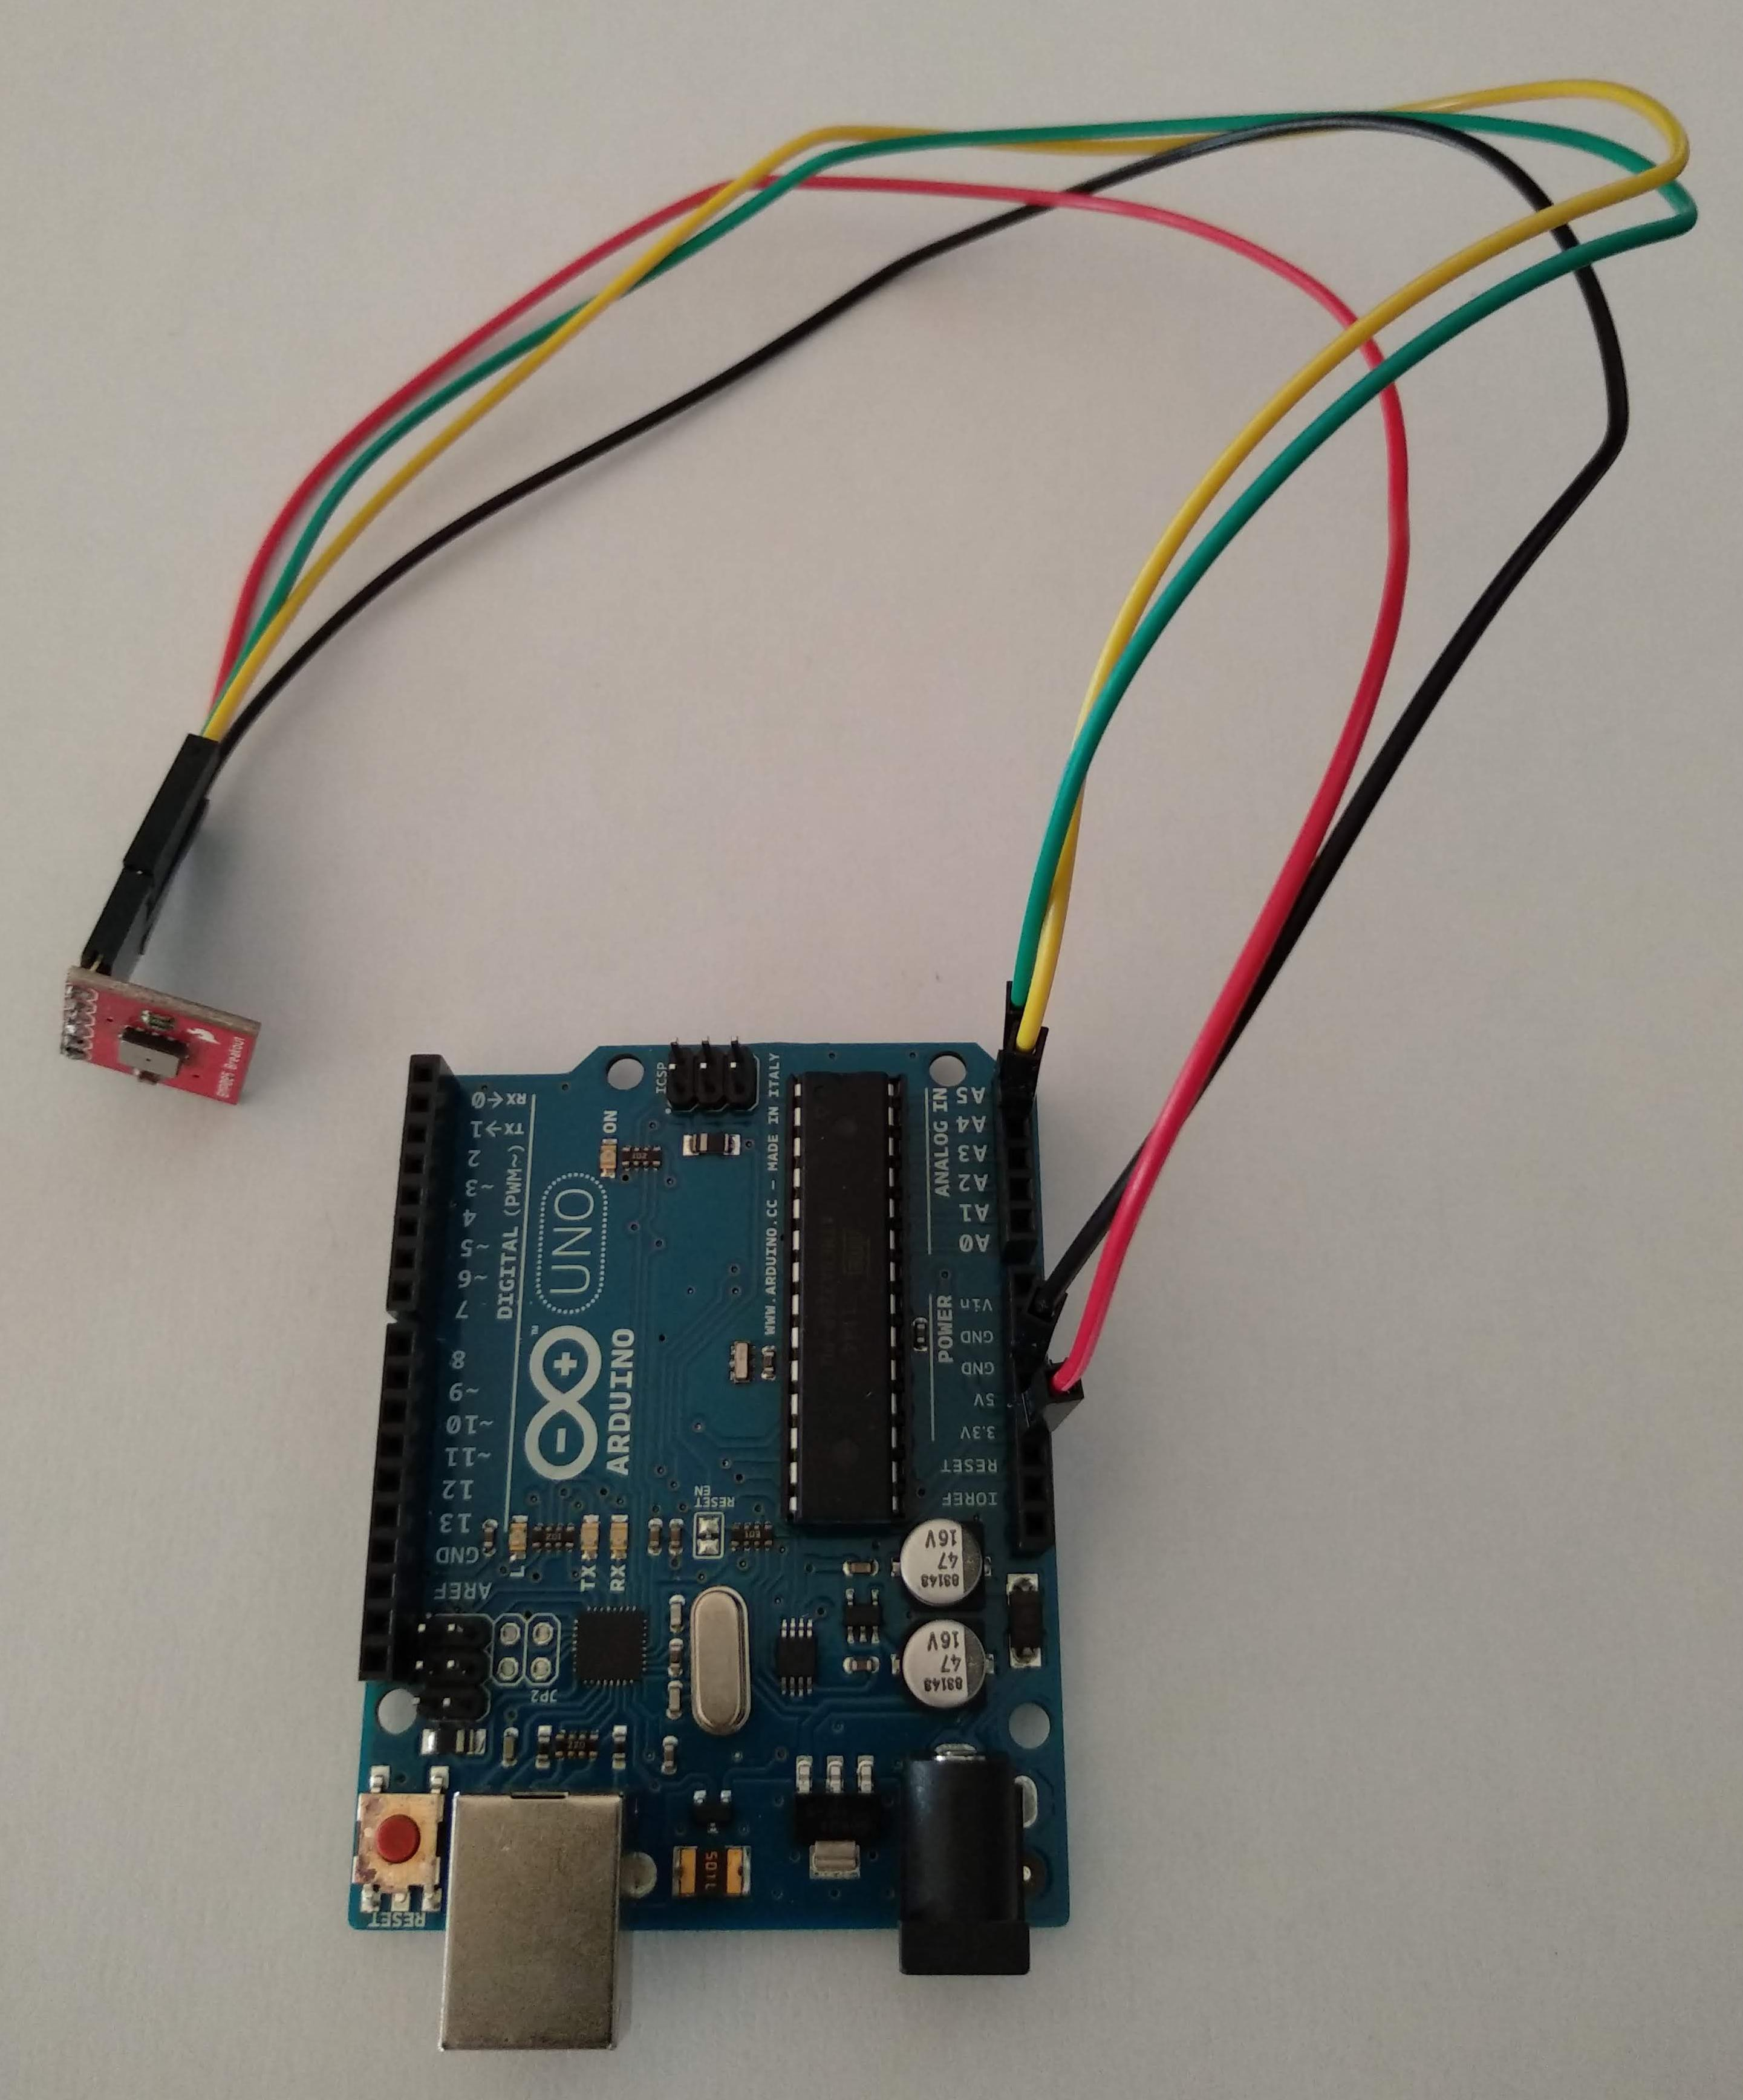
\includegraphics[scale=0.2,keepaspectratio=true]{./imagenes/sensor-presion.jpg}
    % sensor-presion.jpg: 640x480 pixel, 72dpi, 22.58x16.93 cm, bb=0 0 640 480
    \caption{Sensor de presión}
    \label{figura:SensorPresion}
   \end{figure}
   
   Ademáis de definir a súa interface pública (figura 
   \ref{figura:InterfaceSensorPresion}) para a obtención da presión e un
   ficheiro de proba (figura \ref{figura:TestSensorPresion}) para validar a
   implementación completa posterior. \\
   
   \begin{figure}[htbp]
    \centering
    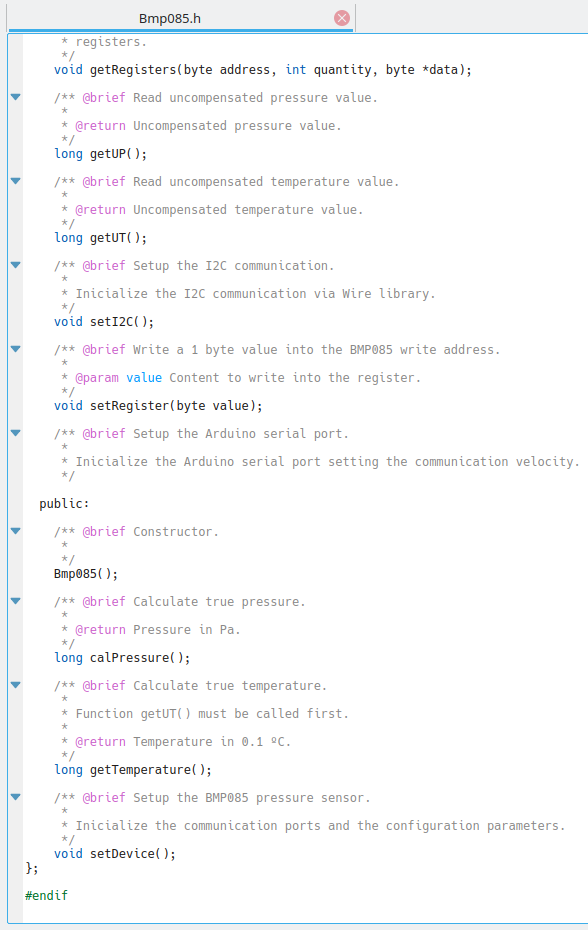
\includegraphics[scale=0.8,keepaspectratio=true]{./imagenes/interface-sensor-presion.png}
    % interface-sensor-presion.png: 640x480 pixel, 72dpi, 22.58x16.93 cm, bb=0 0 640 480
    \caption{Interface do sensor de presión}
    \label{figura:InterfaceSensorPresion}
   \end{figure}
   
   \begin{figure}[htbp]
    \centering
    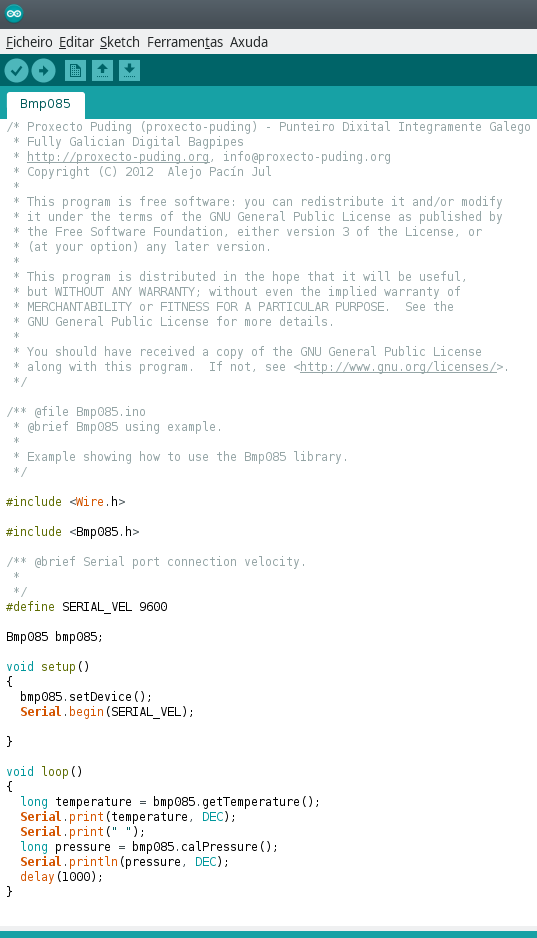
\includegraphics[scale=0.8,keepaspectratio=true]{./imagenes/test-sensor-presion.png}
    % test-sensor-presion.png: 640x480 pixel, 72dpi, 22.58x16.93 cm, bb=0 0 640 480
    \caption{Ficheiro de proba do sensor de presión}
    \label{figura:TestSensorPresion}
   \end{figure}
   
   O turno seguinte foi para os sensores capacitivos. Neste caso, o que
   precisamos saber é cáles están acesos en cada momento, de maneira que
   poidamos facer \textit{pattern matching} contra a configuración da gaita e
   saber se teriamos algún son asociado a dita dixitación, para posteriormente
   reproducilo. \\
   
   Como se pode ver na imaxe, conectouse a unha placa Arduino Uno empregando
   o bus I2C do mesmo. \\
  
   \begin{figure}[htbp]
    \centering
    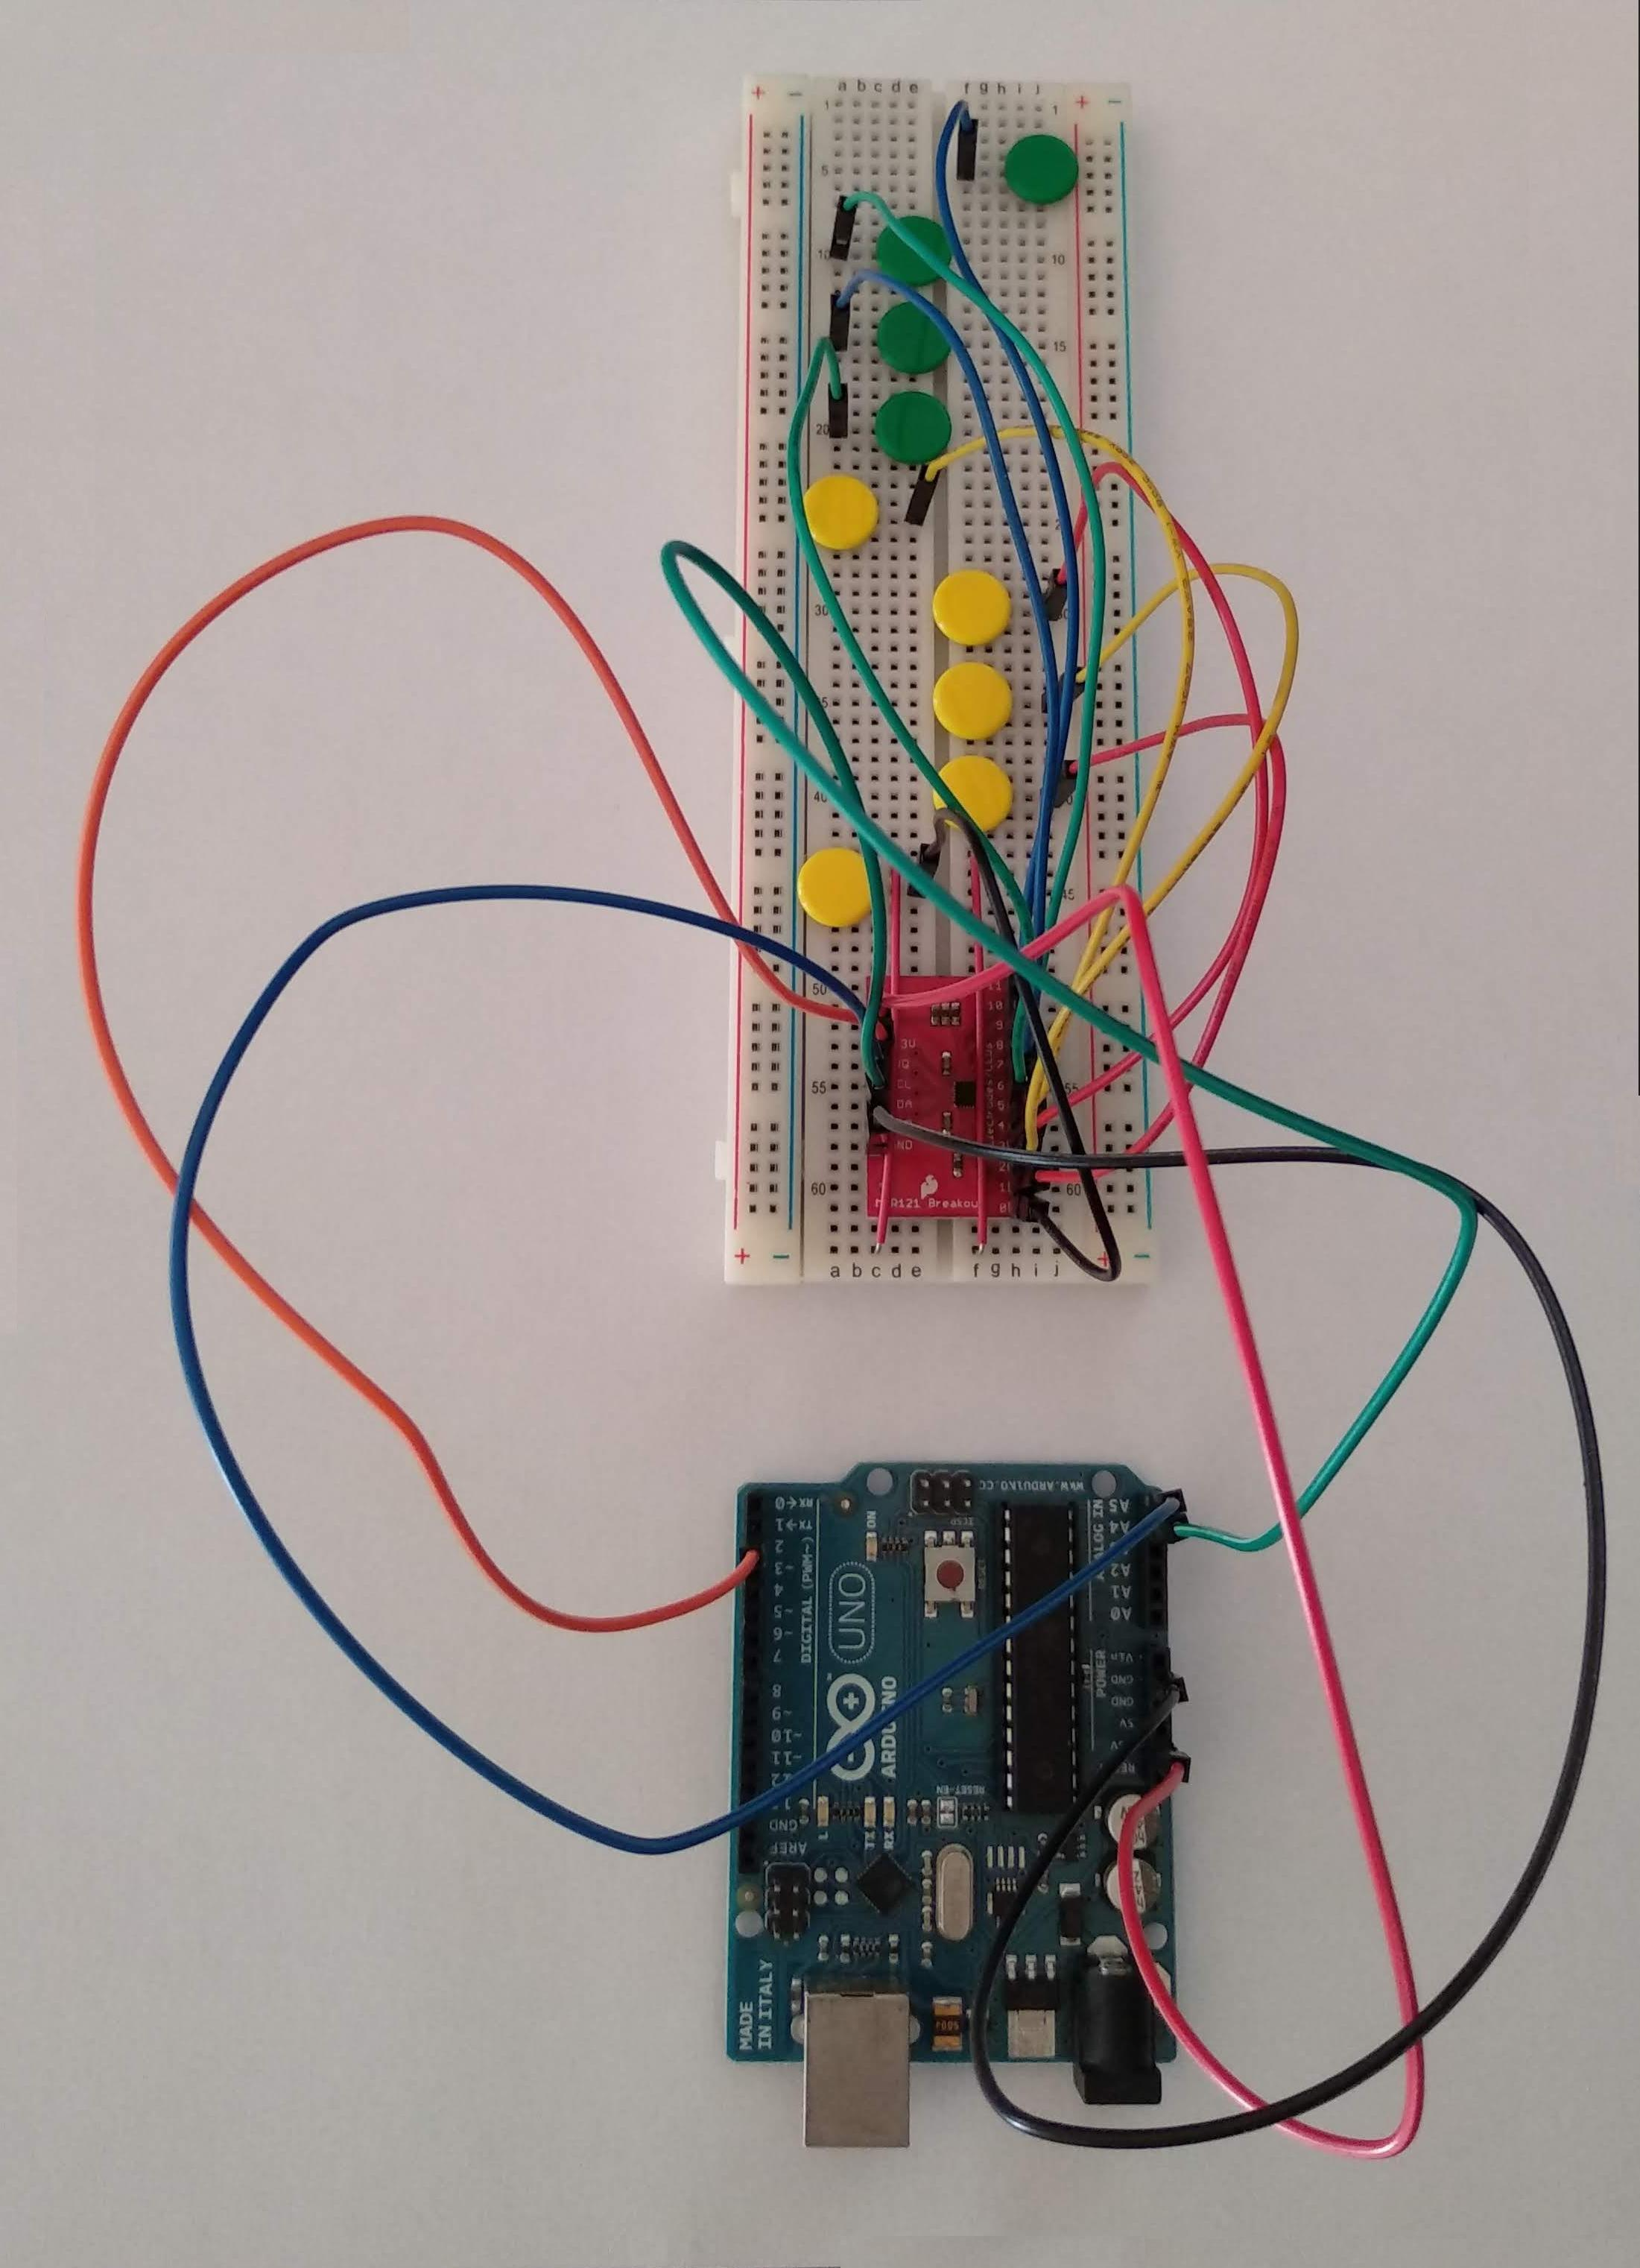
\includegraphics[scale=0.2,keepaspectratio=true]{./imagenes/sensores-capacitivos.jpg}
    % sensores-capacitivos.jpg: 640x480 pixel, 72dpi, 22.58x16.93 cm, bb=0 0 640 480
    \caption{Sensores capacitivos}
    \label{figura:SensoresCapacitivos}
   \end{figure}
   
   Ademáis de definir a súa interface pública (figura 
   \ref{figura:InterfaceSensoresCapacitivos}) para a obtención da dixitación e
   un ficheiro de proba (figura \ref{figura:TestSensoresCapacitivos}) para
   validar a implementación completa posterior. \\
   
   \begin{figure}[htbp]
    \centering
    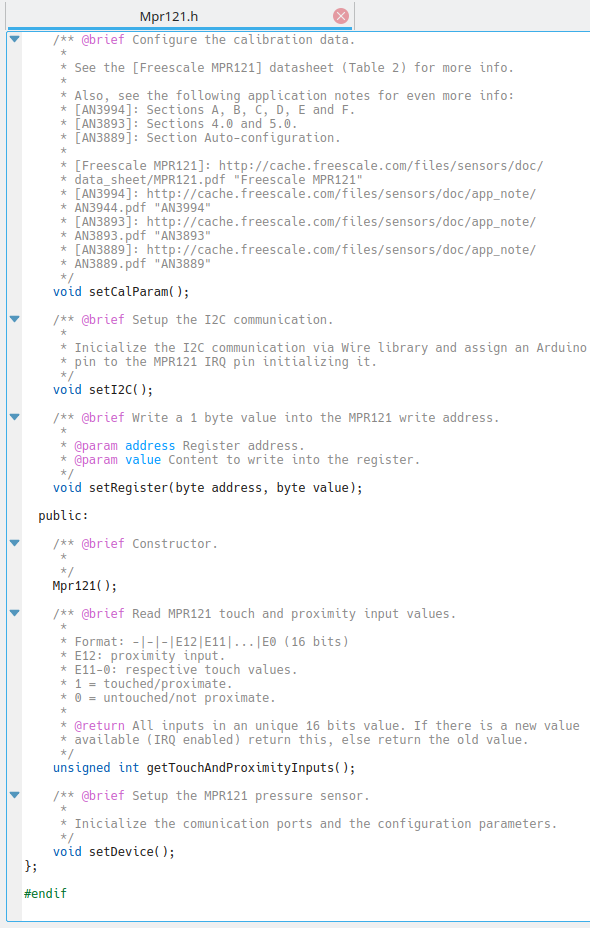
\includegraphics[scale=0.8,keepaspectratio=true]{./imagenes/interface-sensores-capacitivos.png}
    % interface-sensores-capacitivos.png: 640x480 pixel, 72dpi, 22.58x16.93 cm, bb=0 0 640 480
    \caption{Interface dos sensores capacitivos}
    \label{figura:InterfaceSensoresCapacitivos}
   \end{figure}
   
   \begin{figure}[htbp]
    \centering
    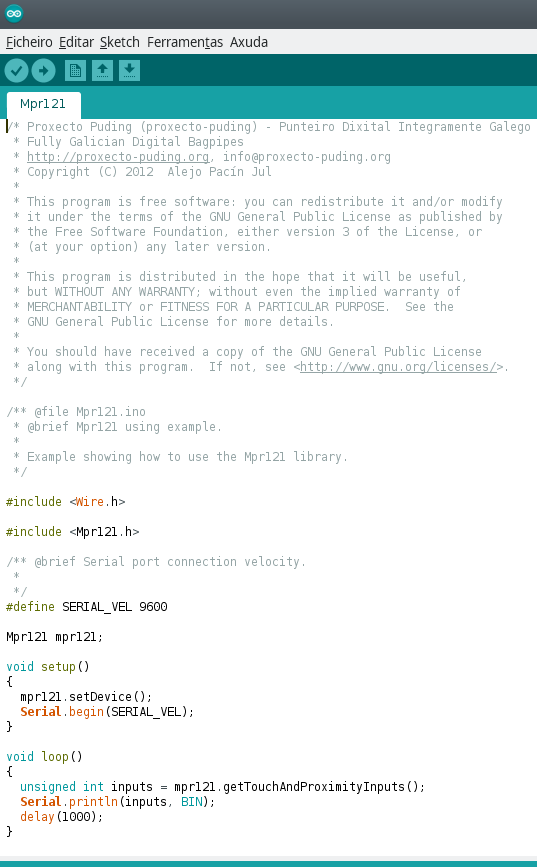
\includegraphics[scale=0.8,keepaspectratio=true]{./imagenes/test-sensores-capacitivos.png}
    % test-sensores-capacitivos.png: 640x480 pixel, 72dpi, 22.58x16.93 cm, bb=0 0 640 480
    \caption{Ficheiro de proba dos sensores capacitivos}
    \label{figura:TestSensoresCapacitivos}
   \end{figure}
   
   Para rematar cos periféricos, procedeuse co lector de tarxetas. Neste caso o
   que precisamos é poder ler e almacenar a configuración variable do
   dispositivo, de maneira que sexa independente e única para cada un dos
   mesmos. \\
   
   Como se pode ver na imaxe, conectouse a unha placa Arduino Uno empregando
   o porto UART do mesmo. \\
  
   \begin{figure}[htbp]
    \centering
    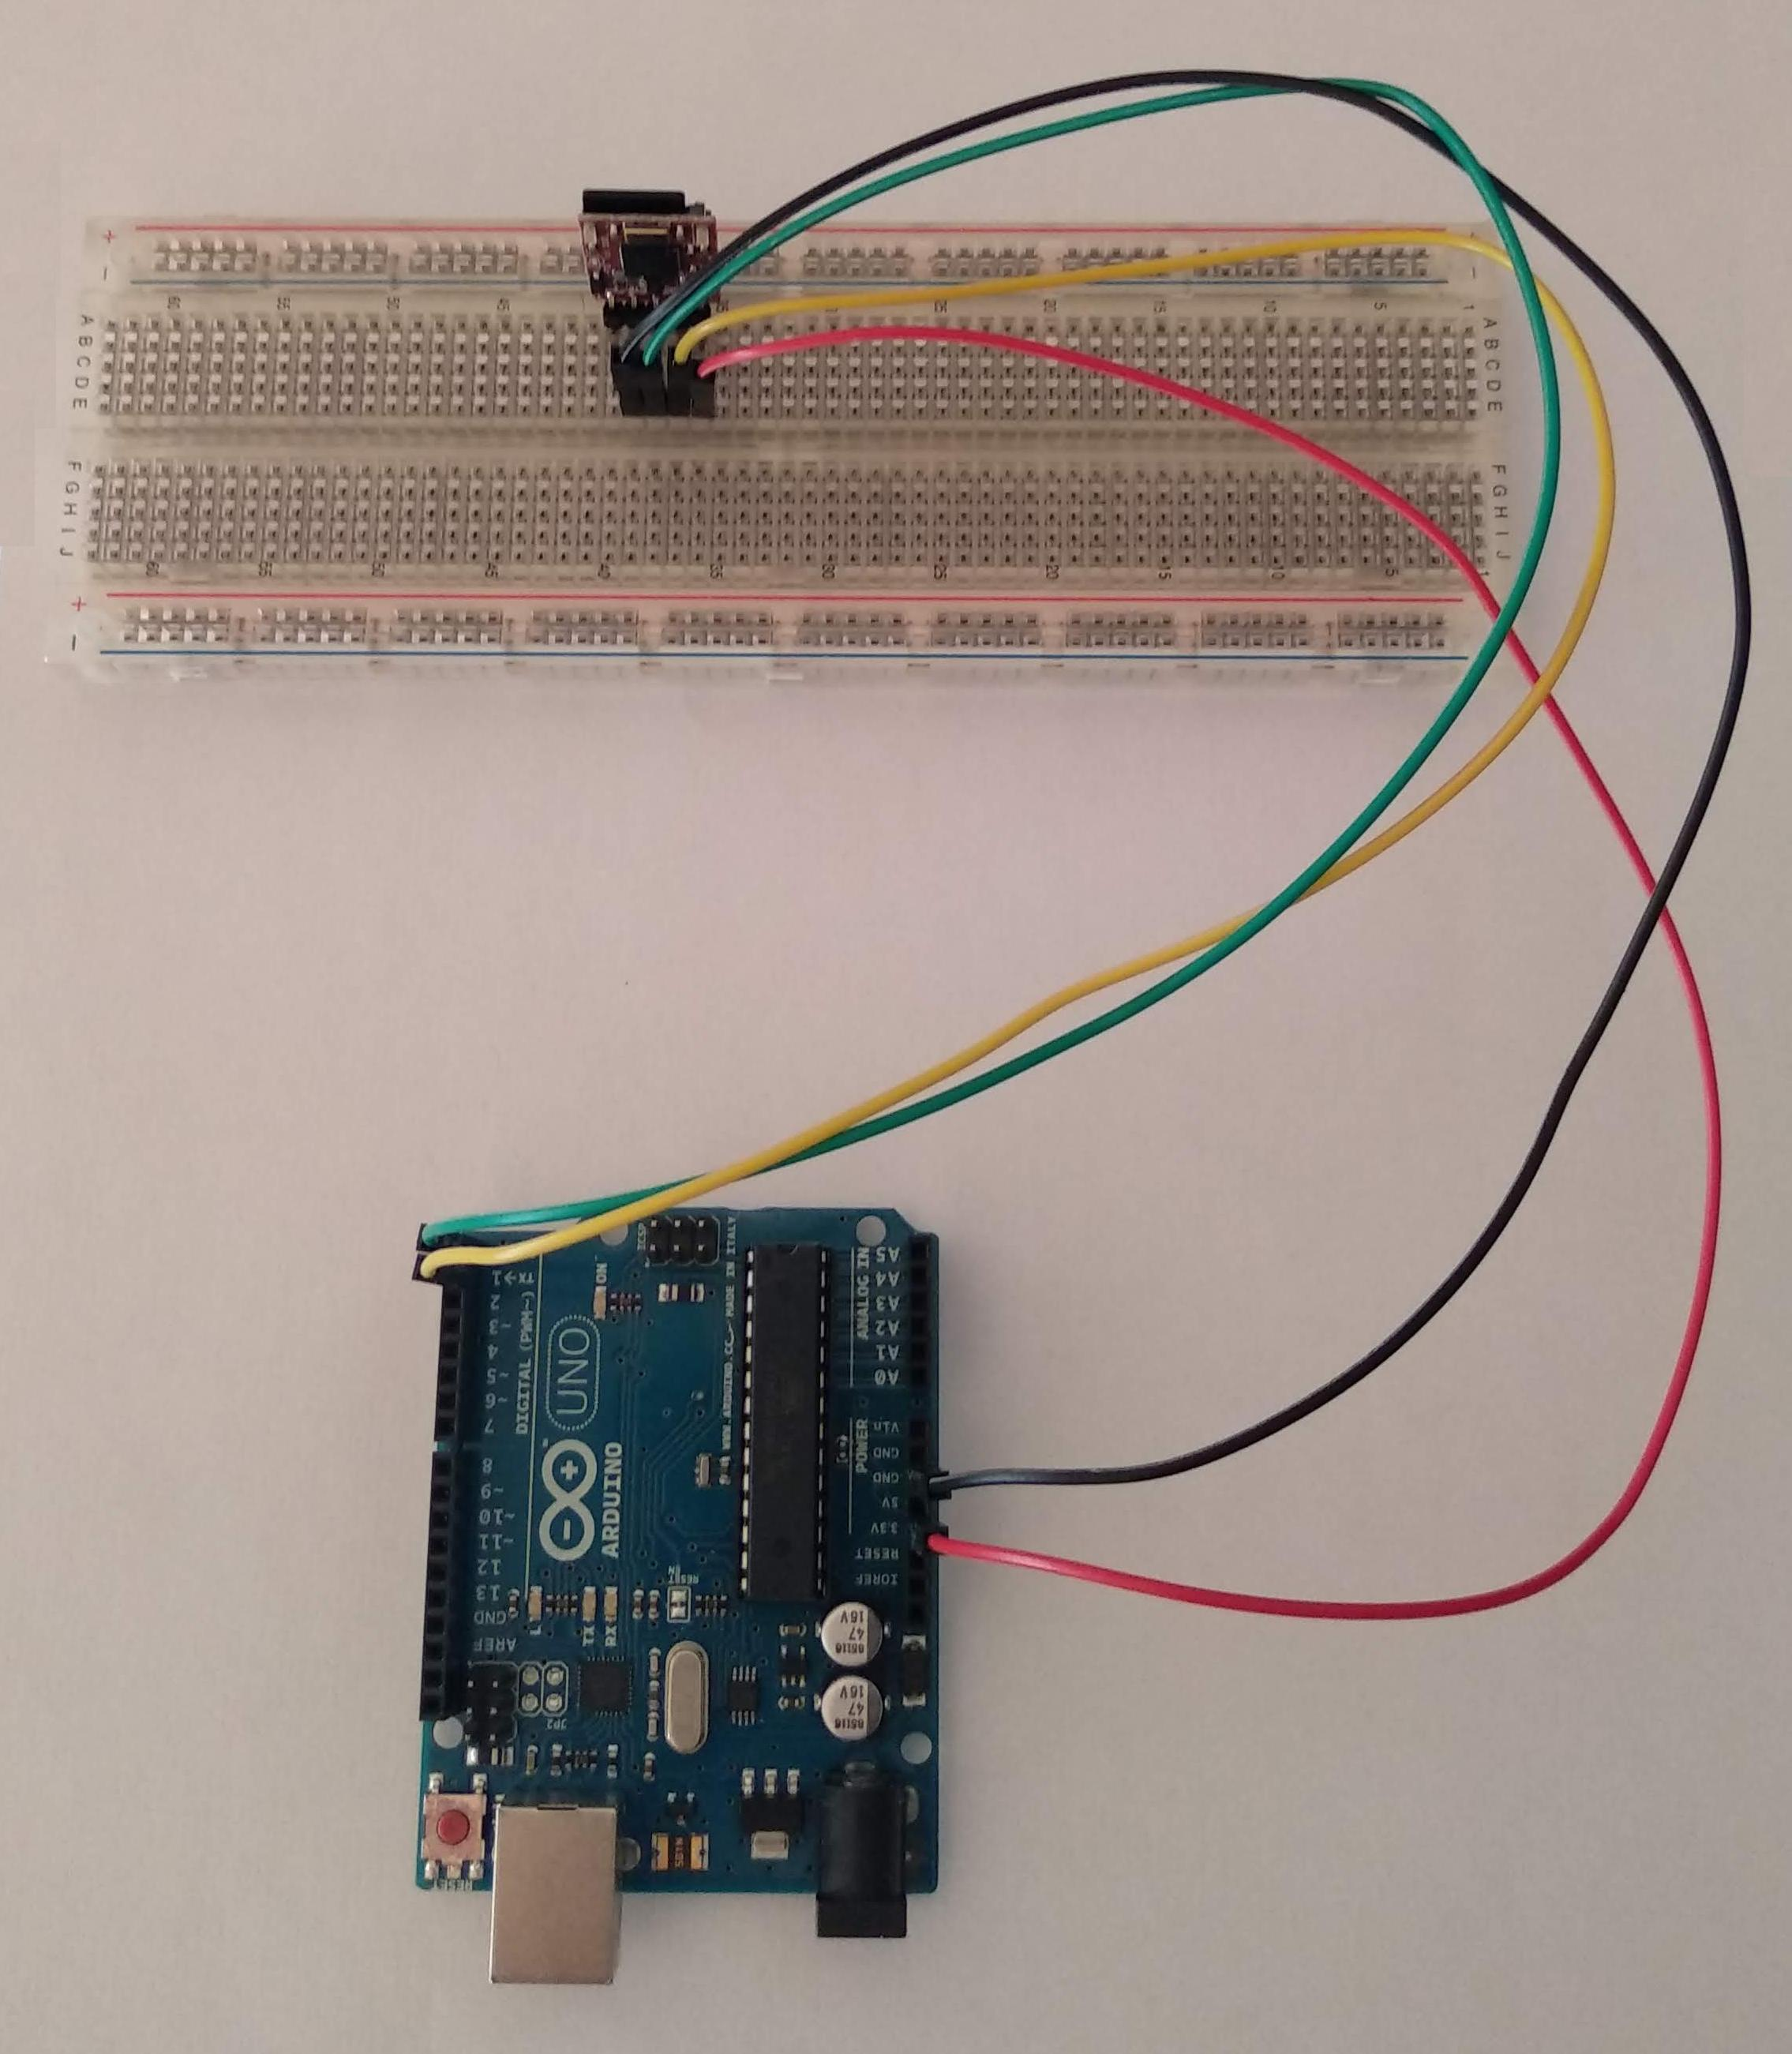
\includegraphics[scale=0.2,keepaspectratio=true]{./imagenes/lector-tarxetas.jpg}
    % lector-tarxetas.jpg: 640x480 pixel, 72dpi, 22.58x16.93 cm, bb=0 0 640 480
    \caption{Lector de tarxetas}
    \label{figura:LectorTarxetas}
   \end{figure}
   
   Ademáis de definir a súa interface pública (figura 
   \ref{figura:InterfaceLectorTarxetas}) para a obtención da configuración e un
   ficheiro de proba (figura \ref{figura:TestLectorTarxetas}) para validar a
   implementación completa posterior. \\
   
   \begin{figure}[htbp]
    \centering
    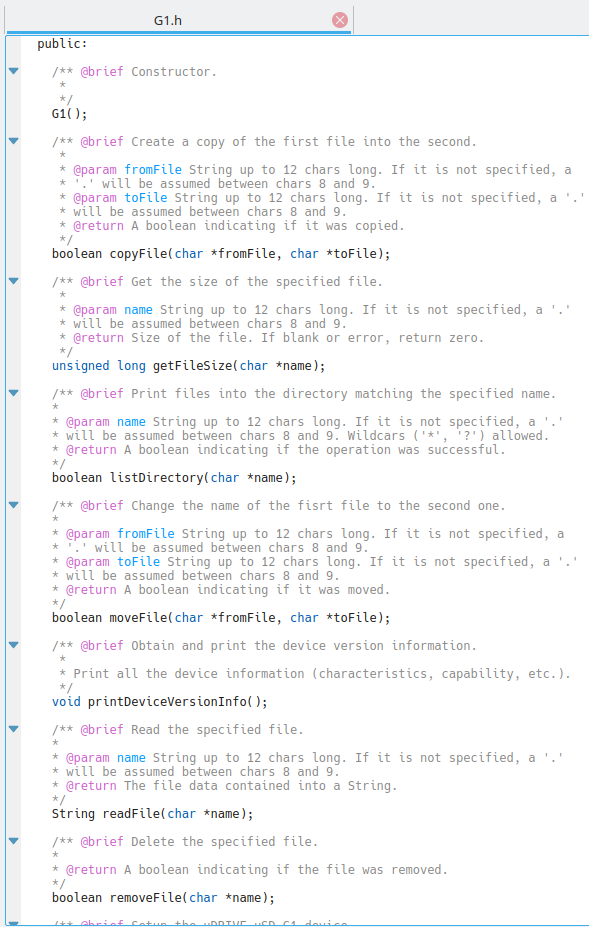
\includegraphics[scale=0.8,keepaspectratio=true]{./imagenes/interface-lector-tarxetas.png}
    % interface-lector-tarxetas.png: 640x480 pixel, 72dpi, 22.58x16.93 cm, bb=0 0 640 480
    \caption{Interface do lector de tarxetas}
    \label{figura:InterfaceLectorTarxetas}
   \end{figure}
   
   \begin{figure}[htbp]
    \centering
    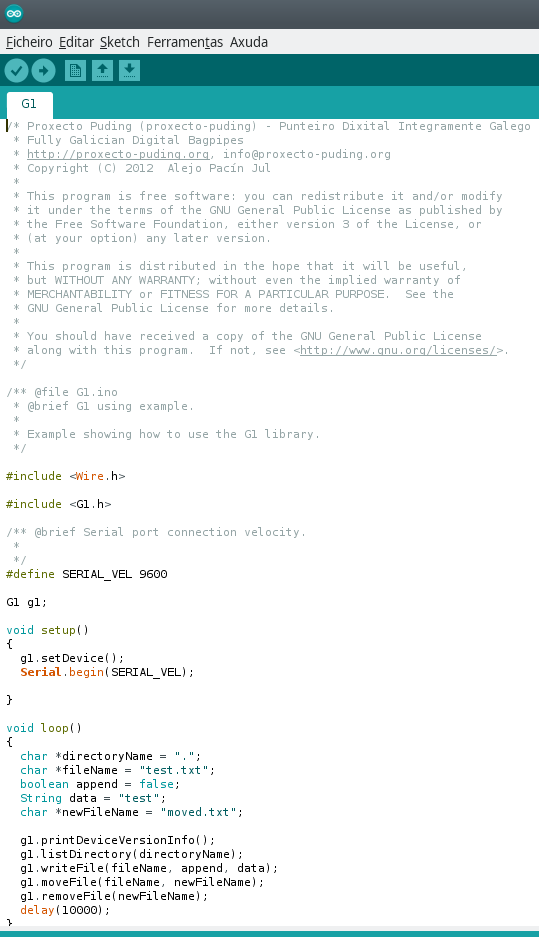
\includegraphics[scale=0.8,keepaspectratio=true]{./imagenes/test-lector-tarxetas.png}
    % test-lector-tarxetas.png: 640x480 pixel, 72dpi, 22.58x16.93 cm, bb=0 0 640 480
    \caption{Ficheiro de proba do lector de tarxetas}
    \label{figura:TestLectorTarxetas}
   \end{figure}

   \paragraph{Encapsulamento do hardware}
   
   Debido a atoparse nunha situación temperá do prototipado físico, o
   encapsulamento do hardware realizouse da maneira máis leve posible, dada a
   necesidade de poder montar e desmontar a vontade durante as probas. \\
   
   Como pode comprobarse nas imaxes do apartado anterior, o único elemento
   encapsulado por completo sería o router e o resto estaría ó aire, facendo uso
   de cables de prototipado para evitar ter que soldar e desoldar durante as
   probas. \\
   
   Ademáis, cada un dos periféricos foi montado por separado ata a integración
   completa do hardware, logo da correcta implementación, verificación e
   validación do mesmo.

  \subsubsection{Prototipo software}
  
  Para a o prototipo software operacional tiramos do prototipo deseñado na fase
  anterior e dos diagramas UML relacionados.

   \paragraph{Desenvolvemento do prototipo}
   
   No tocante ó desenvolvemento do software, contamos con dúas partes ben
   diferenciadas:
   
   \begin{itemize}
    \item O firmware do dispositivo.
    \item E a aplicación de configuración.
   \end{itemize}
   
   Como o firmware do dispositivo xa o tratamos na sección anterior, neste
   apartado centrarémonos no desenvolvemento dun prototipo operacional da
   aplicación de configuración. \\
   
   Como xa comentamos anteriormente, para ilo tiramos dos deseños das pantallas
   e do UML do prototipo da fase de deseño. Combinando os mesmos e facendo uso
   da lóxica de negocio obtida na fase de análise, chegouse a un deseño UML máis
   detallado (figura \ref{figura:DesenoNivelIntermedio}, onde se incluíron os
   servizos necesarios para dar cobertura a dita lóxica. \\
   
   \begin{figure}[htbp]
    \centering
    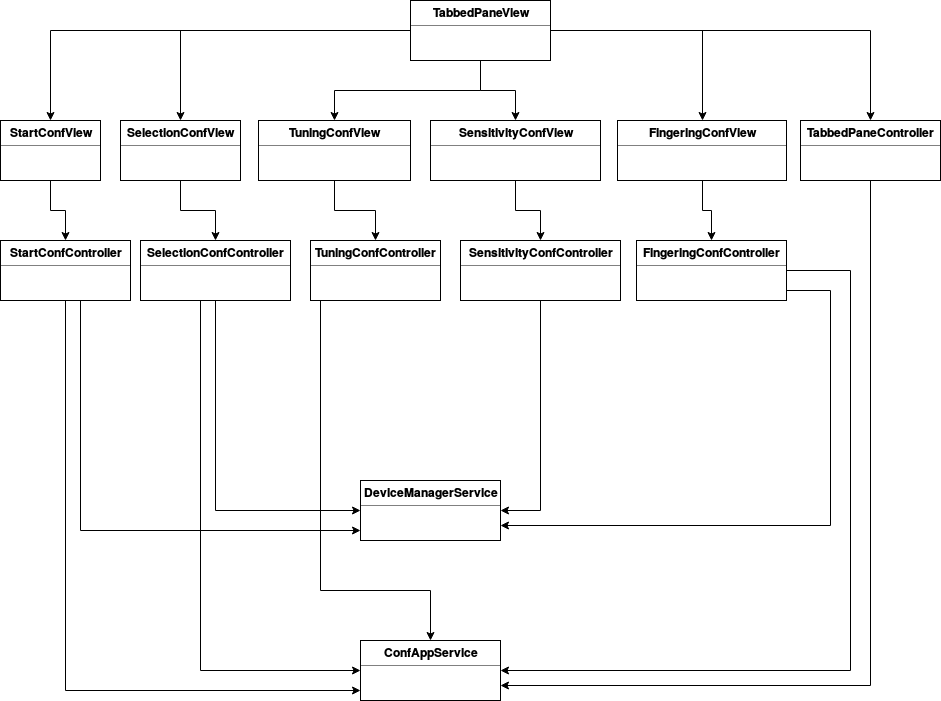
\includegraphics[scale=0.6, angle=90, keepaspectratio=true]{./imagenes/deseno-ni.png}
    % deseno-ni.png: 640x480 pixel, 72dpi, 22.58x16.93 cm, bb=0 0 640 480
    \caption{Deseño de nivel intermedio}
    \label{figura:DesenoNivelIntermedio}
   \end{figure}
   
   Ditos servizos son:
   
   \begin{itemize}
    \item O servizo de dispositivos, encargado de xestionar todo o relacionado
        cos dispositivos hardware en uso: detección, comunicación, etc.
    \item O servizo de configuración, encargado de xestionar todo o relacionado
        coa mesma.
   \end{itemize}
   
   Aplicando BDD e baseándonos na interacción do usuario coas pantallas fóronse
   definindo os distintos casos de uso e a representación conceptual das
   das entidades do modelo para o seu uso polos distintos servizos. \\
   
   A interface do servizo de dispositivos quedou como reflexan as figuras
   \ref{figura:ServizoDispositivos1} a \ref{figura:ServizoDispositivos4}. \\
   
   \begin{figure}[htbp]
    \centering
    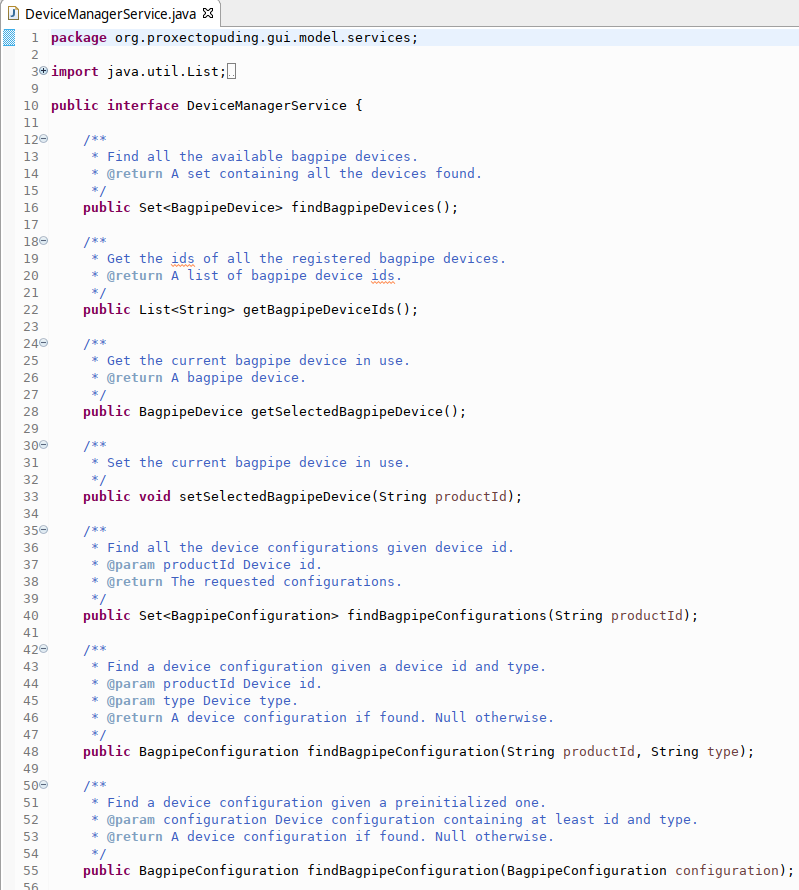
\includegraphics[scale=0.6, keepaspectratio=true]{./imagenes/servizo-dispositivos-1.png}
    % servizo-dispositivos-1.png: 640x480 pixel, 72dpi, 22.58x16.93 cm, bb=0 0 640 480
    \caption{Servizo de dispositivos}
    \label{figura:ServizoDispositivos1}
   \end{figure}
   
   \begin{figure}[htbp]
    \centering
    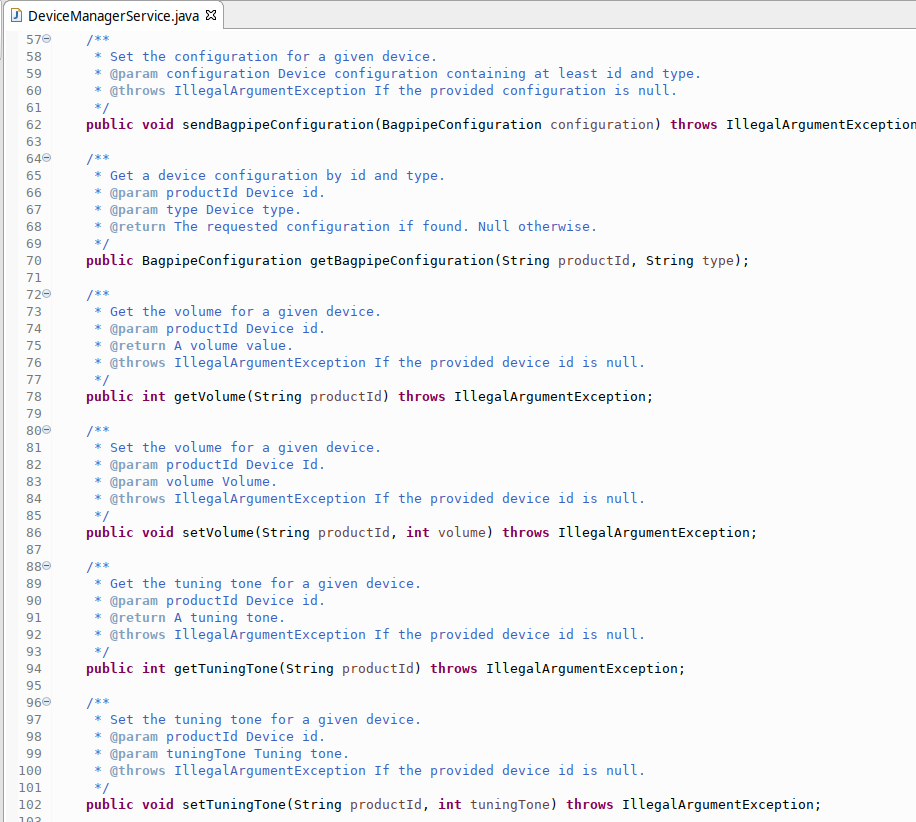
\includegraphics[scale=0.6, keepaspectratio=true]{./imagenes/servizo-dispositivos-2.png}
    % servizo-dispositivos-2.png: 640x480 pixel, 72dpi, 22.58x16.93 cm, bb=0 0 640 480
    \caption{Servizo de dispositivos}
    \label{figura:ServizoDispositivos2}
   \end{figure}
   
   \begin{figure}[htbp]
    \centering
    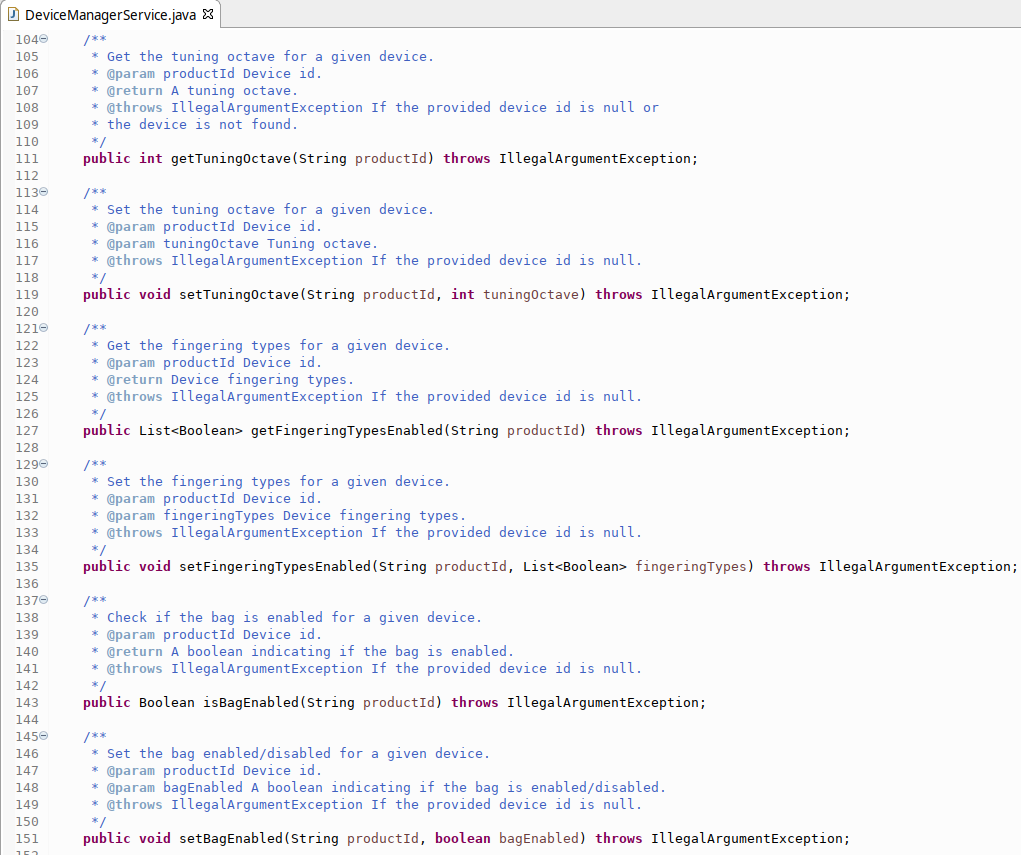
\includegraphics[scale=0.6, keepaspectratio=true]{./imagenes/servizo-dispositivos-3.png}
    % servizo-dispositivos-3.png: 640x480 pixel, 72dpi, 22.58x16.93 cm, bb=0 0 640 480
    \caption{Servizo de dispositivos}
    \label{figura:ServizoDispositivos3}
   \end{figure}
   
   \begin{figure}[htbp]
    \centering
    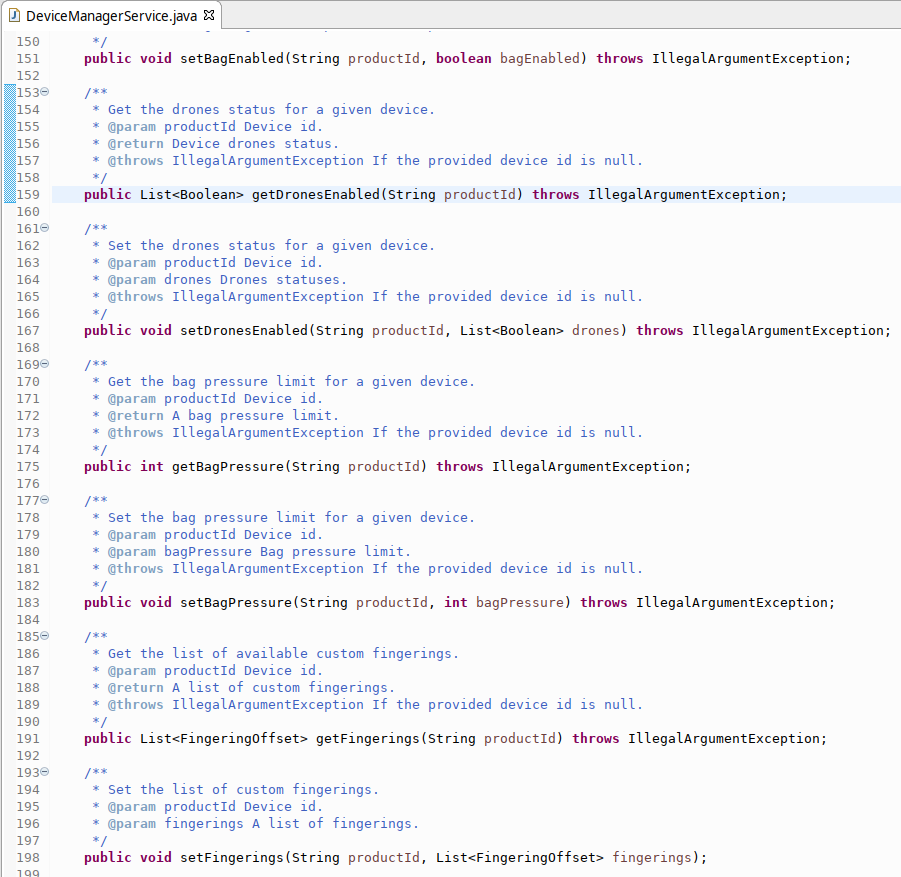
\includegraphics[scale=0.6, keepaspectratio=true]{./imagenes/servizo-dispositivos-4.png}
    % servizo-dispositivo-4s.png: 640x480 pixel, 72dpi, 22.58x16.93 cm, bb=0 0 640 480
    \caption{Servizo de dispositivos}
    \label{figura:ServizoDispositivos4}
   \end{figure}
   
   A interface do servizo de configuración quedou como reflexan as figuras
   \ref{figura:ServizoConfiguracion1} a \ref{figura:ServizoConfiguracion7}. \\
   
   \begin{figure}[htbp]
    \centering
    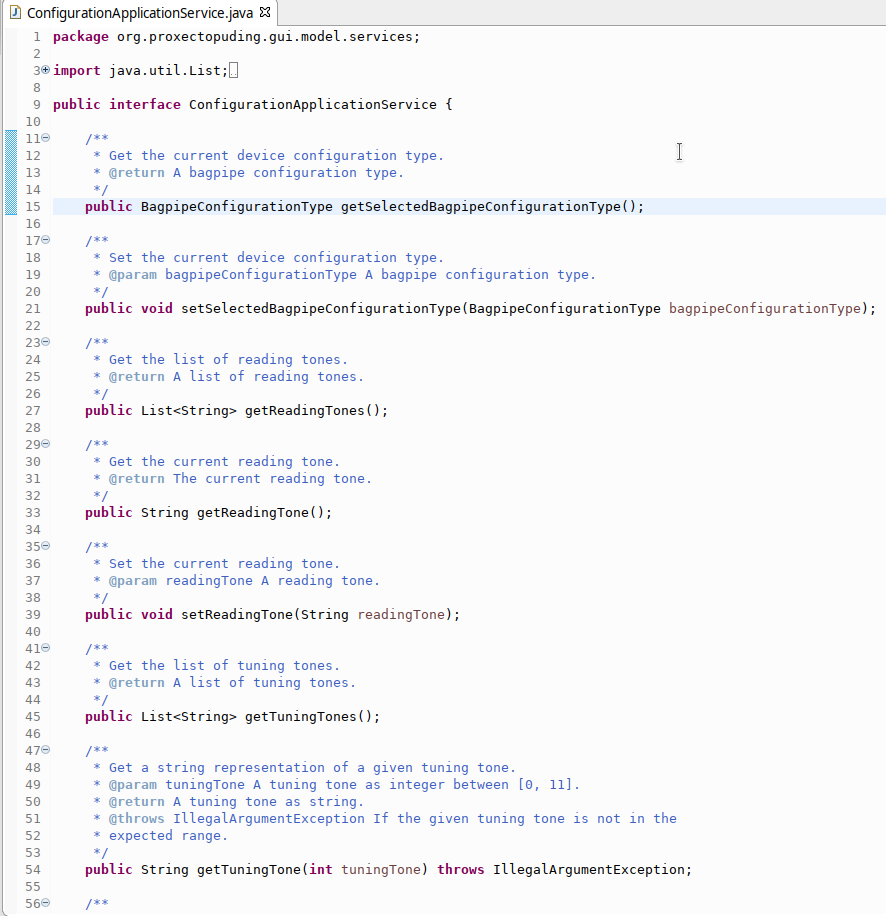
\includegraphics[scale=0.6, keepaspectratio=true]{./imagenes/servizo-configuracion-1.png}
    % servizo-configuracion-1.png: 640x480 pixel, 72dpi, 22.58x16.93 cm, bb=0 0 640 480
    \caption{Servizo de configuración}
    \label{figura:ServizoConfiguracion1}
   \end{figure}
   
   \begin{figure}[htbp]
    \centering
    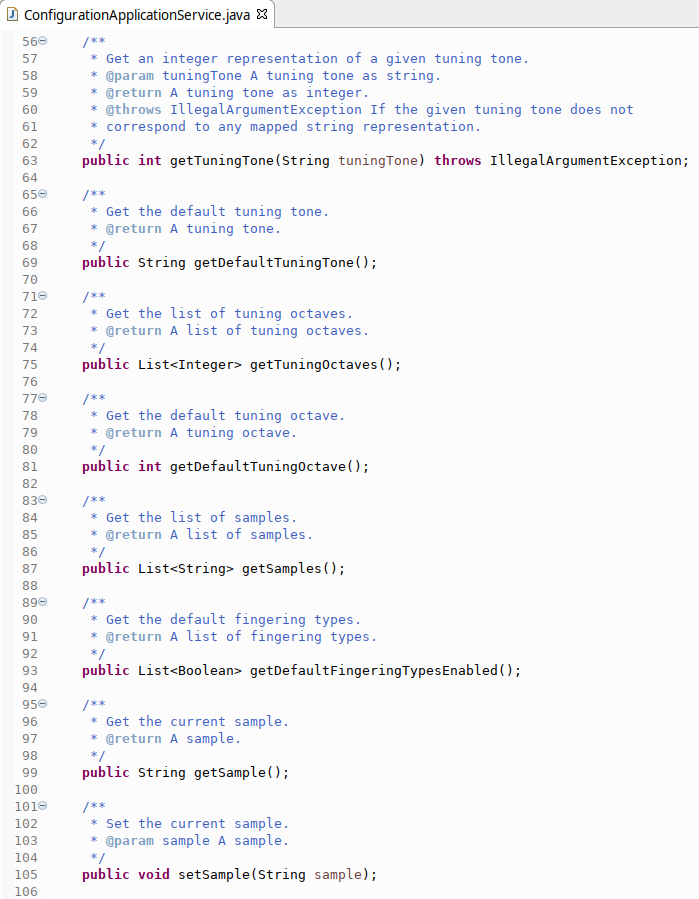
\includegraphics[scale=0.6, keepaspectratio=true]{./imagenes/servizo-configuracion-2.png}
    % servizo-configuracion-2.png: 640x480 pixel, 72dpi, 22.58x16.93 cm, bb=0 0 640 480
    \caption{Servizo de configuración}
    \label{figura:ServizoConfiguracion2}
   \end{figure}
   
   \begin{figure}[htbp]
    \centering
    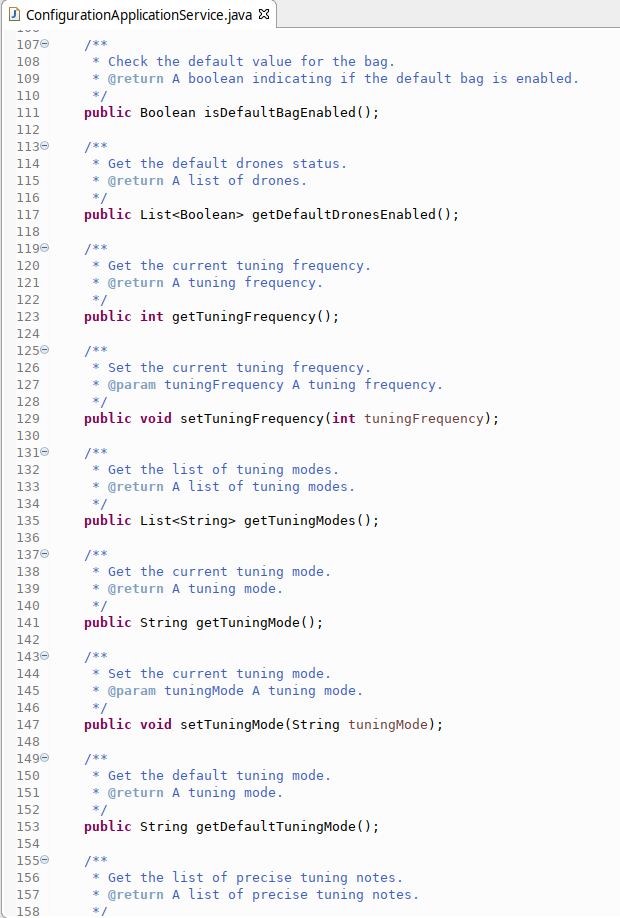
\includegraphics[scale=0.6, keepaspectratio=true]{./imagenes/servizo-configuracion-3.png}
    % servizo-configuracion-3.png: 640x480 pixel, 72dpi, 22.58x16.93 cm, bb=0 0 640 480
    \caption{Servizo de configuración}
    \label{figura:ServizoConfiguracion3}
   \end{figure}
   
   \begin{figure}[htbp]
    \centering
    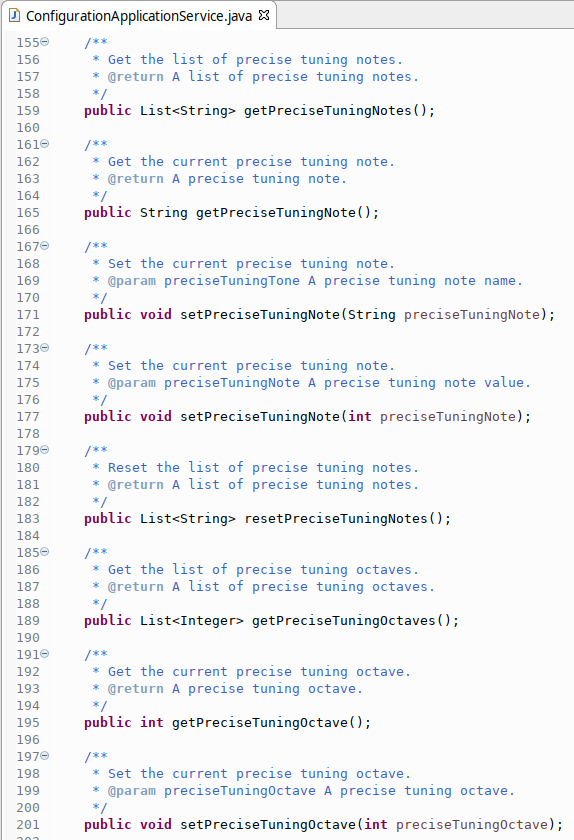
\includegraphics[scale=0.6, keepaspectratio=true]{./imagenes/servizo-configuracion-4.png}
    % servizo-configuracion-4.png: 640x480 pixel, 72dpi, 22.58x16.93 cm, bb=0 0 640 480
    \caption{Servizo de configuración}
    \label{figura:ServizoConfiguracion4}
   \end{figure}
   
   \begin{figure}[htbp]
    \centering
    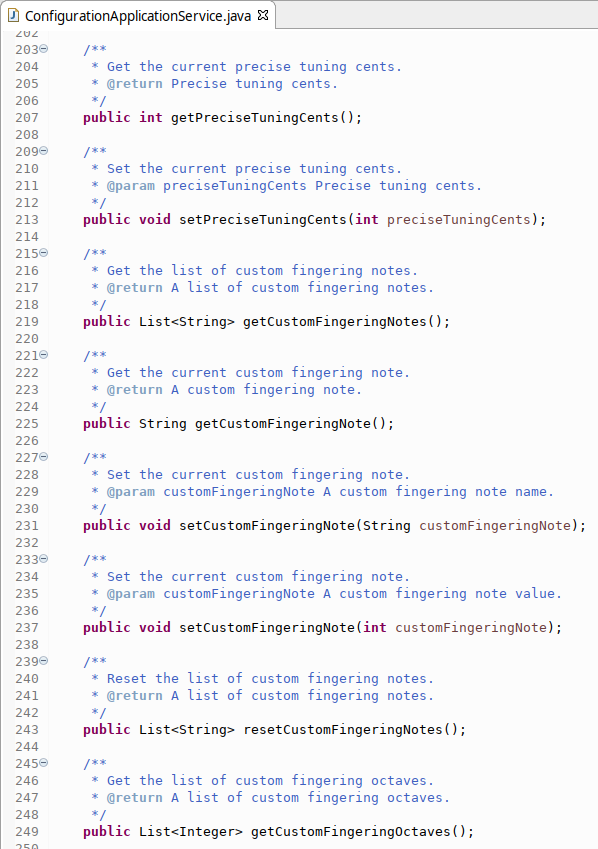
\includegraphics[scale=0.6, keepaspectratio=true]{./imagenes/servizo-configuracion-5.png}
    % servizo-configuracion-5.png: 640x480 pixel, 72dpi, 22.58x16.93 cm, bb=0 0 640 480
    \caption{Servizo de configuración}
    \label{figura:ServizoConfiguracion5}
   \end{figure}
   
   \begin{figure}[htbp]
    \centering
    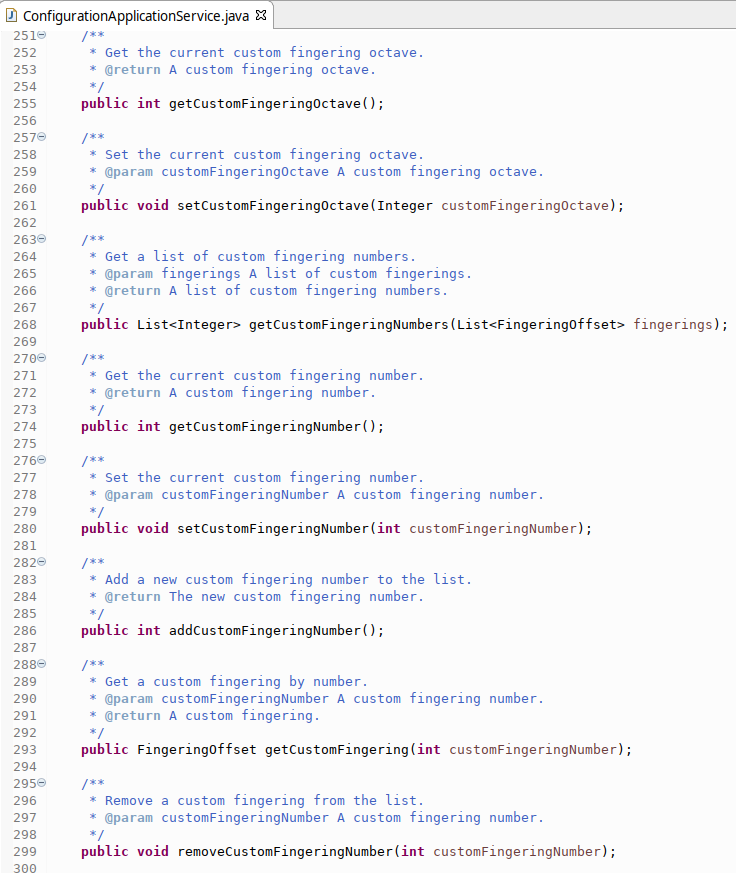
\includegraphics[scale=0.6, keepaspectratio=true]{./imagenes/servizo-configuracion-6.png}
    % servizo-configuracion-6.png: 640x480 pixel, 72dpi, 22.58x16.93 cm, bb=0 0 640 480
    \caption{Servizo de configuración}
    \label{figura:ServizoConfiguracion6}
   \end{figure}
   
   \begin{figure}[htbp]
    \centering
    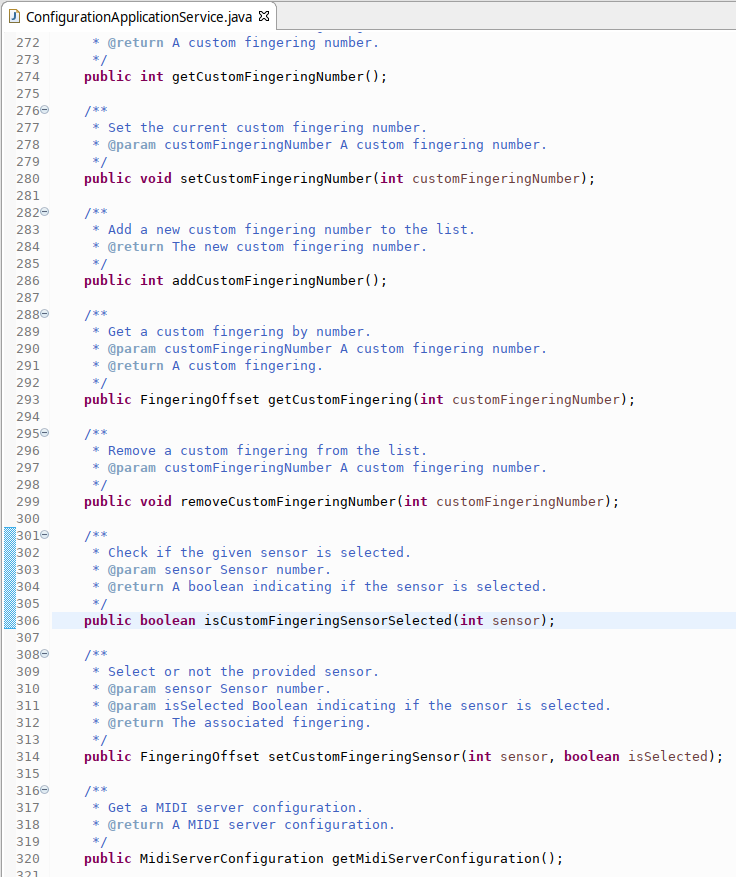
\includegraphics[scale=0.6, keepaspectratio=true]{./imagenes/servizo-configuracion-7.png}
    % servizo-configuracion71.png: 640x480 pixel, 72dpi, 22.58x16.93 cm, bb=0 0 640 480
    \caption{Servizo de configuración}
    \label{figura:ServizoConfiguracion7}
   \end{figure}
   
   Como se pode apreciar nas interfaces dos servizos, as principais entidades
   resultantes do modelo son o dispositivo, os distintos tipos de configuración
   do mesmo e o servidor MIDI, que quedarían como amosan as figuras 
   \ref{figura:BagpipeDevice} a \ref{figura:MidiServerConfiguration}. \\
   
   \begin{figure}[htbp]
    \centering
    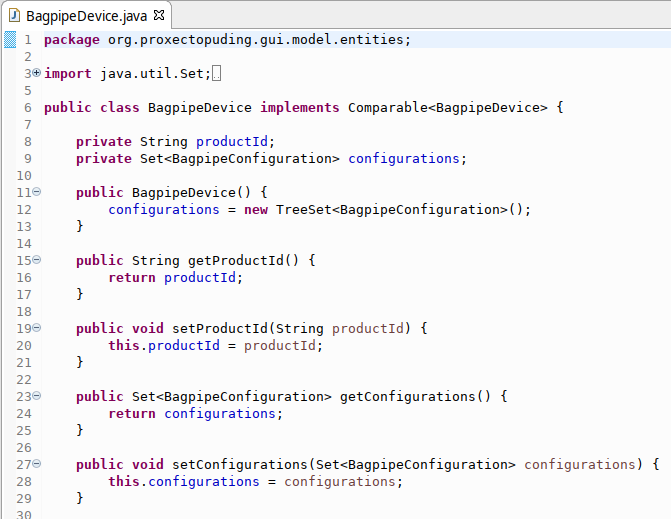
\includegraphics[scale=0.6, keepaspectratio=true]{./imagenes/bagpipe-device.png}
    % bagpipe-device.png: 640x480 pixel, 72dpi, 22.58x16.93 cm, bb=0 0 640 480
    \caption{Dispositivo}
    \label{figura:BagpipeDevice}
   \end{figure}
   
   \begin{figure}[htbp]
    \centering
    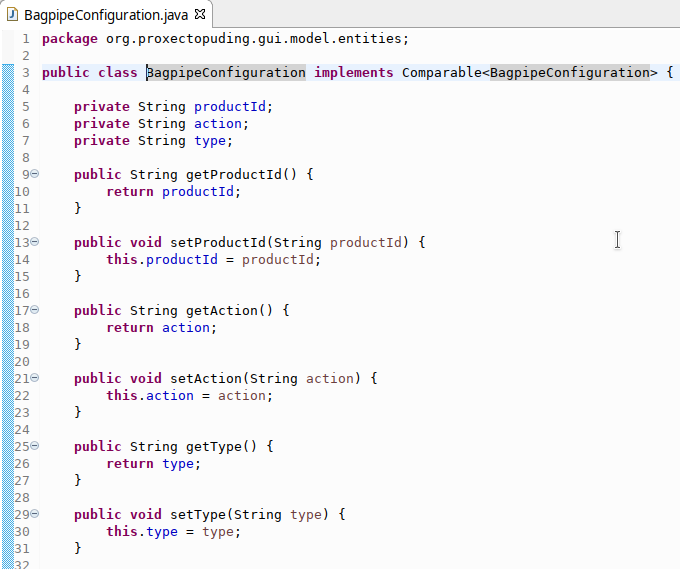
\includegraphics[scale=0.6, keepaspectratio=true]{./imagenes/bagpipe-configuration.png}
    % bagpipe-configuration.png: 640x480 pixel, 72dpi, 22.58x16.93 cm, bb=0 0 640 480
    \caption{Configuración}
    \label{figura:BagpipeConfiguration}
   \end{figure}
   
   \begin{figure}[htbp]
    \centering
    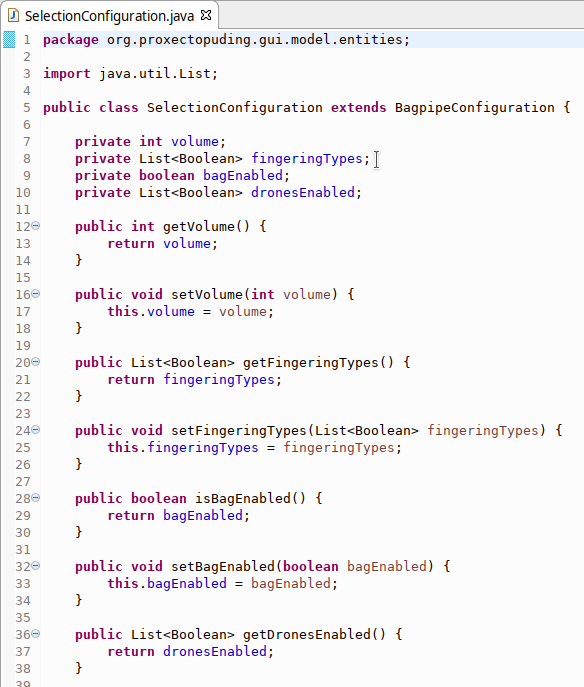
\includegraphics[scale=0.6, keepaspectratio=true]{./imagenes/selection-configuration.png}
    % selection-configuration.png: 640x480 pixel, 72dpi, 22.58x16.93 cm, bb=0 0 640 480
    \caption{Configuración de selección}
    \label{figura:SelectionConfiguration}
   \end{figure}
   
   \begin{figure}[htbp]
    \centering
    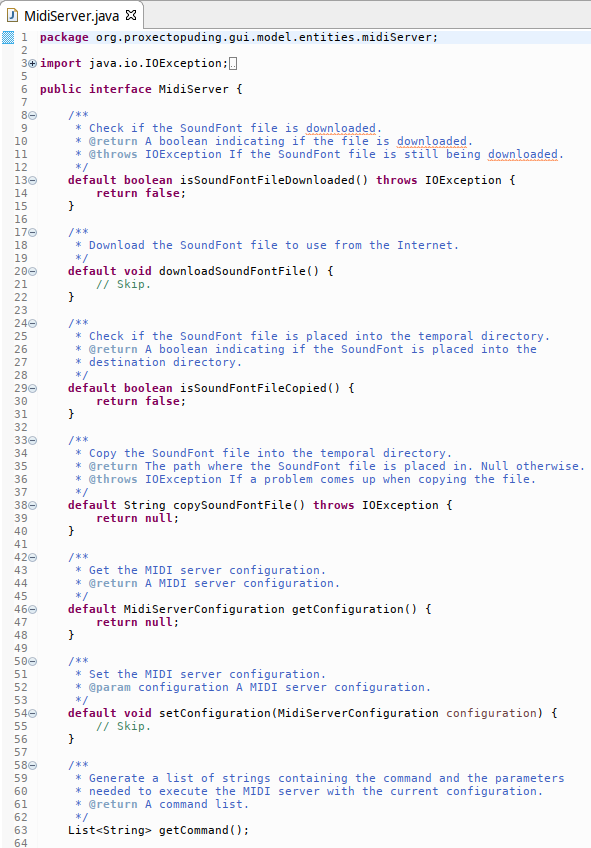
\includegraphics[scale=0.6, keepaspectratio=true]{./imagenes/midi-server.png}
    % midi-server.png: 640x480 pixel, 72dpi, 22.58x16.93 cm, bb=0 0 640 480
    \caption{Servidor MIDI}
    \label{figura:MidiServer}
   \end{figure}
   
   \begin{figure}[htbp]
    \centering
    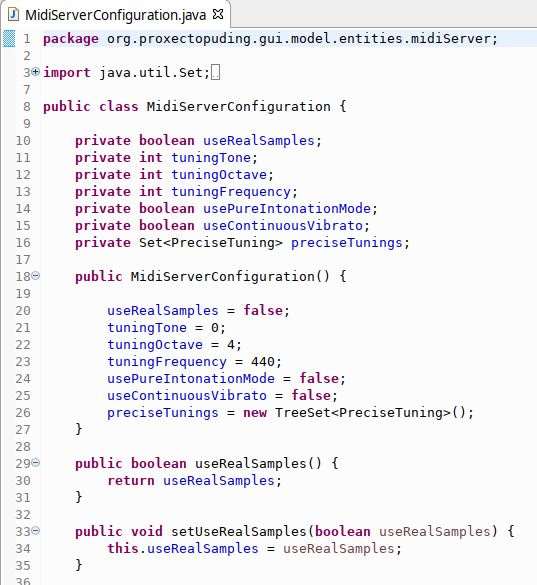
\includegraphics[scale=0.6, keepaspectratio=true]{./imagenes/midi-server-configuration.png}
    % midi-server-configuration.png: 640x480 pixel, 72dpi, 22.58x16.93 cm, bb=0 0 640 480
    \caption{Configuración do servidor MIDI}
    \label{figura:MidiServerConfiguration}
   \end{figure}
   
   Definidos xa servizos e entidades do modelo, procedeuse a conectar vista e
   modelo a través do controlador, tal e como se indica no UML. Desta maneira
   comprobamos de maneira práctica se encaixaban ven ambas partes e se non
   esqueciamos nada importante que puidese implicar un retraballo severo de
   dectectarse nunha fase posterior.

   \paragraph{Gravación das mostras}
   
   Debido á cantidade de horas a invertir neste apartado, entre a gravación das
   mostras e a xeración da fonte de son e á dispoñibilidade de outras fontes xa
   dispoñibles públicamente, aínda que de menor calidade, decidiuse adiar este
   apartado a unha fase posterior dada a pouca relevancia académica do mesmo e
   invertir ditas horas en apartados de maior calado.

\section{Desenvolvemento e validación do seguinte nivel do producto}

 \subsection{Simulacións, modelos e programas de proba}
 
 As probas realizadas neste nivel do producto consistiron inicialmente en
 realizar as mesmas probas da fase anterior sobre os novos prototipos para
 verificar que a implementación cumpría coa especificación de requisitos e de
 que non pasabamos nada por alto. \\
 
 Posteriormente, de maneira máis formal e seguindo a metodoloxía de
 desenvolvemento citada (BDD/TDD), definíronse unha serie de probas funcionais
 a nivel de unidade, integración e aceptación a nivel de servizos e para ambos
 sistemas, de maneira que se puidesen validar e verificar o seu funcionamento
 tanto antes coma despois de implementar a lóxica do mesmos. Ditas probas serán
 explicadas en detalle ó final deste capítulo. \\

 \subsection{Deseño detallado}

  \subsubsection{Deseño hardware}
  
  Contando xa cun deseño formal e detallado do producto hardware dende fases
  anteriores e non tendo detectado novos problemas, decidimos seguir empregando
  o \textit{Prototipo 3 hardware} (figura \ref{figura:Prototipo3HardwareBB1})
  coma deseño do mesmo.

  \subsubsection{Deseño software}
  
  Baseándose no deseño de nivel medio do prototipo software operacional
  (figura \ref{figura:DesenoNivelIntermedio}) e nas carencias e melloras
  detectadas durante as probas realizadas sobre a implementación de dito
  prototipo, chegouse a un deseño de nivel medio máis detallado onde se
  incluíron novos servizos que agrupan funcionalidades relacionadas que ven non
  estaban reflexadas de maneira explícita ou teñen un peso máis secundario. \\
  
  Na figura \ref{figura:DesenoBaixoNivel} pode apreciarse o diagrama UML deste
  deseño máis completo.
  
  \begin{figure}[htbp]
    \centering
    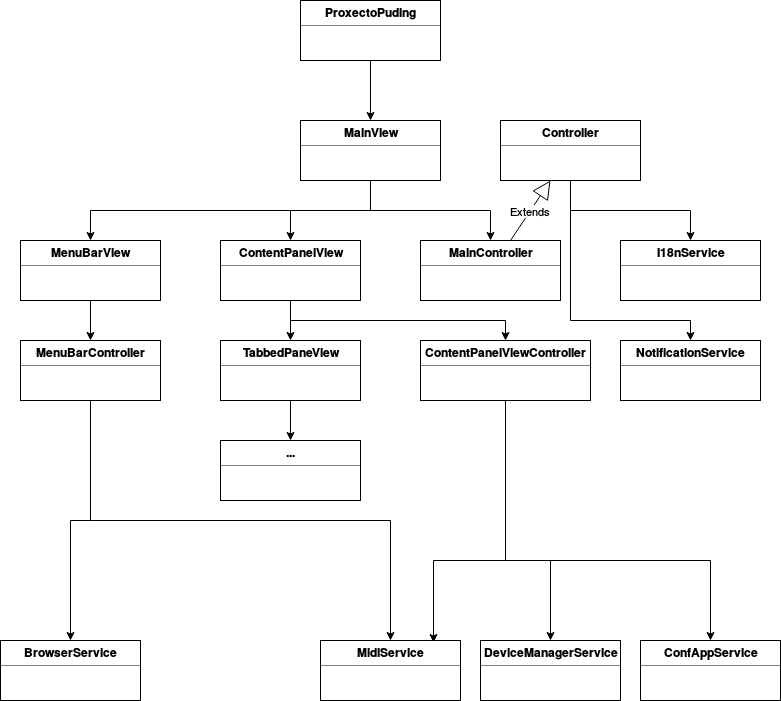
\includegraphics[scale=0.6, keepaspectratio=true]{./imagenes/deseno-bn.png}
    % deseno-bn.png: 640x480 pixel, 72dpi, 22.58x16.93 cm, bb=0 0 640 480
    \caption{Deseño detallado}
    \label{figura:DesenoBaixoNivel}
   \end{figure}
  
  Entre ditos servizos figuran:
   
   \begin{itemize}
    \item O servizo de internacionalización, encargado de proporcionar as
        mensaxes da aplicación no idioma do usuario.
    \item O servizo de notificacións, encargado de xestionar a comunciación
        entre as distintas partes da interface mediante eventos.
    \item O servizo de navegación web, que permite xestionar a apertura da
        documentación da aplicación directamente no navegador do sistema.
    \item O servizo MIDI, que se encarga de xestionar todo o relacionado coas
        operacións sobre o servidor MIDI.
   \end{itemize}
   
   Aplicando BDD e baseándonos na interacción do usuario coas pantallas fóronse
   definindo os distintos casos de uso e a representación conceptual das
   das entidades do modelo para o seu uso polos distintos servizos. \\
   
   A interfaces dos distintos servizos quedaron tal e como reflexan as figuras
   \ref{figura:ServizoI18n} a \ref{figura:ServizoMidi}. \\
   
   \begin{figure}[htbp]
    \centering
    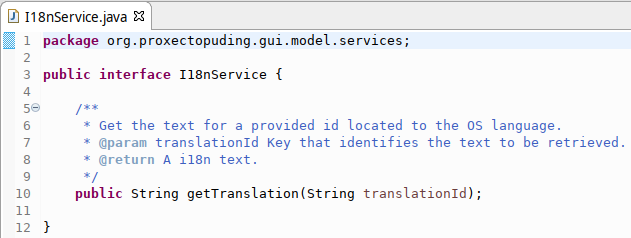
\includegraphics[scale=0.6, keepaspectratio=true]{./imagenes/servizo-i18n.png}
    % servizo-i18n.png: 640x480 pixel, 72dpi, 22.58x16.93 cm, bb=0 0 640 480
    \caption{Servizo de internacionalización}
    \label{figura:ServizoI18n}
   \end{figure}
   
   \begin{figure}[htbp]
    \centering
    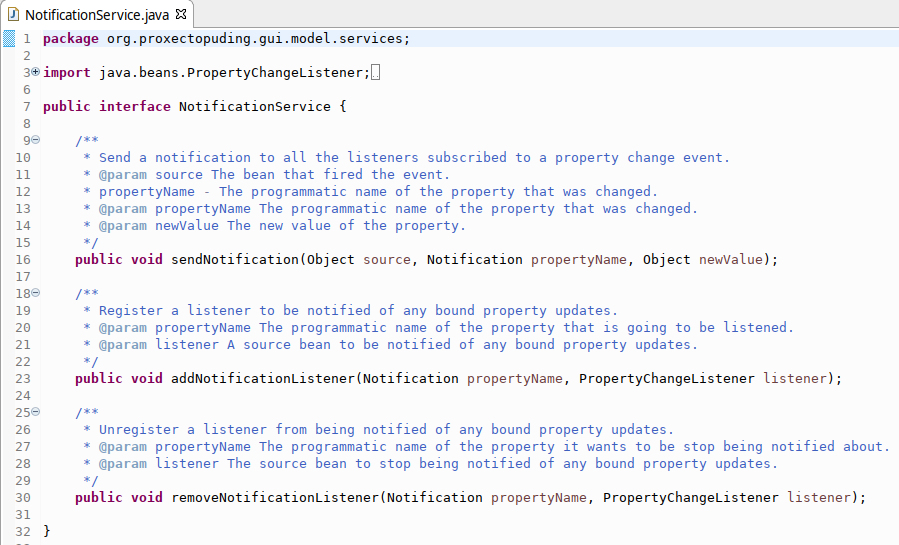
\includegraphics[scale=0.6, keepaspectratio=true]{./imagenes/servizo-notificacions.png}
    % servizo-notificacions.png: 640x480 pixel, 72dpi, 22.58x16.93 cm, bb=0 0 640 480
    \caption{Servizo de notificacións}
    \label{figura:ServizoNotificacions}
   \end{figure}
   
   \begin{figure}[htbp]
    \centering
    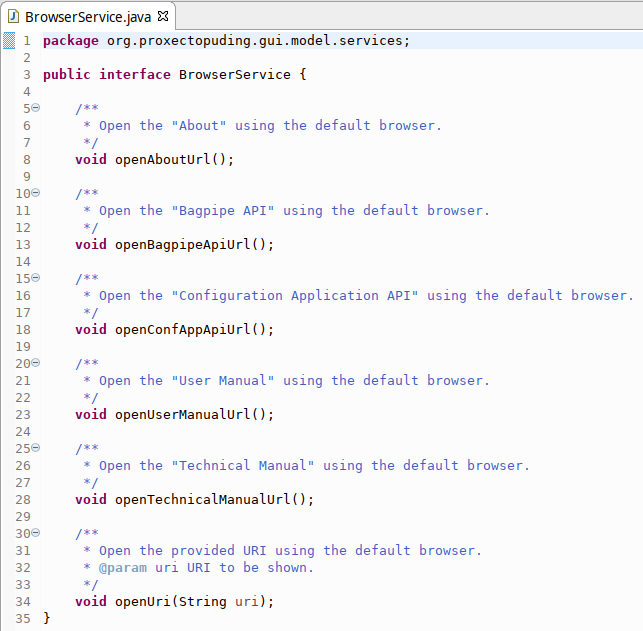
\includegraphics[scale=0.6, keepaspectratio=true]{./imagenes/servizo-navegacion.png}
    % servizo-navegacion.png: 640x480 pixel, 72dpi, 22.58x16.93 cm, bb=0 0 640 480
    \caption{Servizo de navegación web}
    \label{figura:ServizoNavegacion}
   \end{figure}
   
   \begin{figure}[htbp]
    \centering
    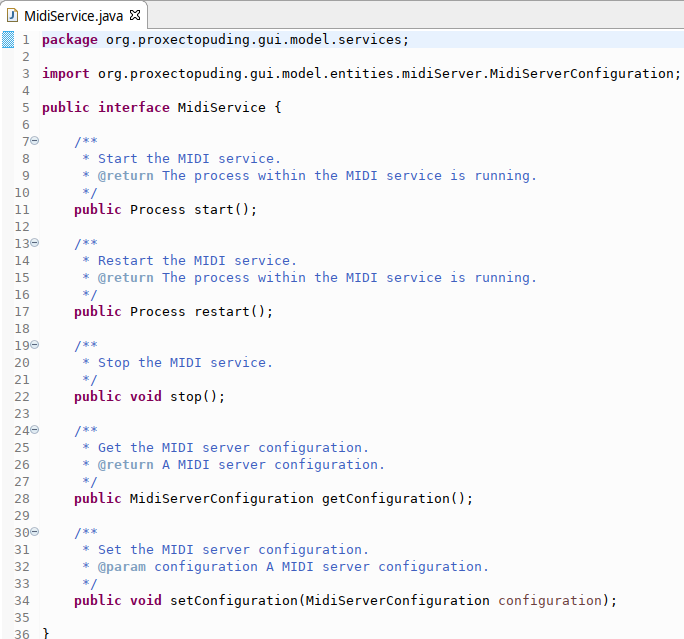
\includegraphics[scale=0.6, keepaspectratio=true]{./imagenes/servizo-midi.png}
    % servizo-midi.png: 640x480 pixel, 72dpi, 22.58x16.93 cm, bb=0 0 640 480
    \caption{Servizo MIDI}
    \label{figura:ServizoMidi}
   \end{figure}
   
   Redefinidos xa servizos e entidades do modelo, procedeuse a reconectar vista
   e modelo a través do controlador facendo uso dos mesmos, tal e como se indica
   no UML. Desta maneira recomprobamos de maneira práctica se encaixaban ven
   ambas partes e se non esqueciamos nada importante que puidese implicar un
   retraballo severo de dectectarse nunha fase posterior.

 \subsection{Ensamblado e codificación}

  \subsubsection{Ensamblado}
  
  Debido a unha serie de razóns de peso (detallados na sección de incidencias),
  descartouse a integración completa e ensamblado de todo o hardware nunha única
  montaxe:
  
  \begin{itemize}
    \item Con respecto á integración, durante a fase final de codificación
        e integración software xurdiron unha serie de problemas que simplemente
        aconsellaron non acoplar todos os compoñentes na mesma montaxe.
    \item Con respecto ó encapsulado, ó non ter toda a montaxe integrada, perde
        a súa razón de ser, ademáis de ser contraproducente mentres non se
        rematen as probas, tal e como se comentou antes. Este sería o paso final
        en calquera caso.
   \end{itemize}

  \subsubsection{Codificación}
  
  Como se comentou con anterioridade, debido á metodoloxía empregada (BDD/TDD),
  a codificación tanto do firmware coma da aplicación de configuración foi o
  último paso de todos, dado que primeiramente se definiron as probas. \\
  
  Unha vez tivemos definidas as probas, para o que fomos en sentido
  \textit{top-down} ata o nivel de servizo, cambiamos o sentido a
  \textit{bottom-up} para facer a implementación dos mesmos en ámbolos casos.
  
   \paragraph{Hardware}
   
   A codificación do firmware do hardware levouse a cabo por partes e de menor
   a maior dificultade:
   
   \begin{itemize}
    \item Sensor de presión.
    \item Sensores capacitivos.
    \item Lector de tarxetas.
    \item Receptor: configuración e reproducción MIDI.
   \end{itemize}
   
   Aínda que a maior dificultade común a todas elas foi a complexidade da
   documentación e a falta dun entorno de desenvolvemento serio. \\
   
   Comezando polo \textbf{sensor de presión}, este caso é a excepción que 
   confirma a regra. Ó ser unha peza desenvolvida por Bosh (compañía moi seria
   en canto a desenvolvemento de sensores), a folla de especificacións
   \cite{BMP085} é impecable. \\
   
    O proceso consistiu en:
    
    \begin{itemize}
    \item Solicitar a lectura da presión.
    \item Definir e ler os rexistros da ROM onde se almacenan os coeficientes de
        calibración do disposito.
    \item Definir e ler os rexistros da ROM onde se almacenan os coeficientes de
        calibración do disposito.
    \item Ler a temperatura sen compensar (4.5 ms).
    \item Definir o modo de lectura da presión e ler a presión sen compensar.
        Como nos interesaba a velocidade e o baixo consumo máis que a precisión,
        optouse polo modo de ultra baixo consumo (4.5 ms), co que se obteñen
        valores bastante desviados, pero como o que precisamos a nivel de lóxica
        de negocio é un valor umbral (ou dous se optamos por un comparador con
        histérese), que o valor sexa máis ou menos real non é o importante.
    \item Calcular a temperatura real aplicando os coeficientes de calibración.
    \item Calcular a presión real aplicando os coeficientes de calibración.
    \item Devolver a presión real, que é o valor que realmente nos interesa,
        invertindo un tempo de arredor de 9 ms, que está por debaixo dos 100 ms
        que se adoitan considerar como tempo real duro para intrumentación MIDI
        e incluso por debaixo dos 10 ms que se considera o óptimo e que serían
        imperceptibles.
   \end{itemize}
   
   Dado que tanto as direccións dos rexistros dos coeficientes de calibración e
   a aplicación dos mesmos e o pseudo-código especificado
   \ref{figura:Bmp085PseudoCodigo} estaban moi ben explicados, foi relativamente
   sinxelo facer funcionar o sensor e que pasase as probas definidas
   anteriormente. Os resultados das mesmas comentaranse no apartado de probas
   unitarias. \\
   
   Finalmente, entre documentación, código e probas, obtivemos un módulo de moi
   baixo nivel en C de arredor de 500 liñas. \\
   
   \begin{figure}[htbp]
    \centering
    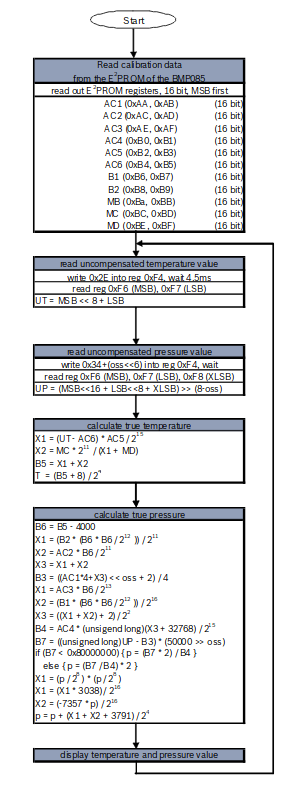
\includegraphics[scale=0.6, keepaspectratio=true]{./imagenes/bmp085-pseudocodigo.png}
    % servizo-midi.png: 640x480 pixel, 72dpi, 22.58x16.93 cm, bb=0 0 640 480
    \caption{Pseudo-código do sensor de presión}
    \label{figura:Bmp085PseudoCodigo}
   \end{figure}
   
   Continuando polos \textbf{sensores capacitivos}, a folla de especificacións
   \cite{MPR121}, de Freescale neste caso, tamén é de calidade, polo que
   facilitou o desenvolvemento. \\
   
   O proceso consistiu en:
    
    \begin{itemize}
    \item Solicitar a lectura da presión mediante I2C.
    \item Definir e ler os rexistros da ROM onde se almacenan as configuracións
        e e valores medidos do disposito.
    \item Ler os valores dos sensores.
    \item Devolver os valores medidos.
   \end{itemize}
   
   A configuración dos rexistros foi de lonxe a parte máis complexa e tediosa.
   Houbo que configurar medio cento de rexistros agrupados nunha decena de
   grupos funcionais e facelo nunha orde concreta, antes de poder facer calquera
   outra operación. \\
   
   En xeral, precisamos obter o valor dos 9 bits/sensores menos significativos
   da placa (que empregaremos para as dixitacións), máis o 13º, sensor virtual
   de presencia (que empregaremos para o vibrato). \\
   
   A lectura dos valores dos sensores realízase primeiro en bruto, sendo pasados
   a continuación por tres filtros de distinto tipo, como se pode apreciar na
   figura \ref{figura:Mpr121Medicion}. \\
   
   \begin{figure}[htbp]
    \centering
    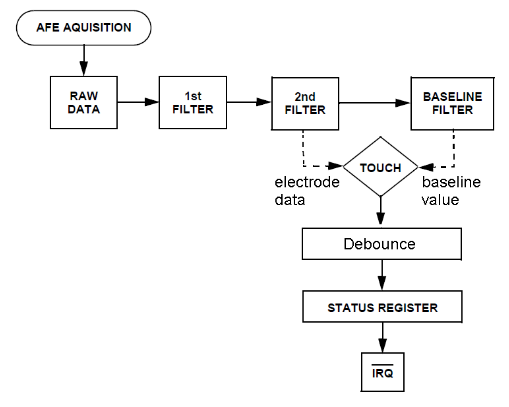
\includegraphics[scale=0.6, keepaspectratio=true]{./imagenes/mpr121-medicion.png}
    % mpr121-medicion.png: 640x480 pixel, 72dpi, 22.58x16.93 cm, bb=0 0 640 480
    \caption{Medición dos sensores capacitivos}
    \label{figura:Mpr121Medicion}
   \end{figure}
   
   O sensor de proximidade é un sensor virtual que calcula o seu valor en
   función do valor dos outros 12 sensores físicos, de maneira que podemos
   empregalo para calcular pequenas variacións ou vibracións dos son en función
   de se hai outros dedos próximos ós sensores que non están sendo empregados
   na dixitación. \\
   
   Outro punto moi importante que descubrimos na folla de especificacións é que
   os sensores son auto-calibrables, polo que o requisito sobre o axuste da
   sensibilidade do sensores, logo de facer probas con distinta xente e vendo
   que os valores eran correctos, quedou cuberto pola parte hardware sen
   necesidade de cubrilo dende o software de configuración, motivo polo que se
   revisou a pantalla de configuración da sensibilidade do punteiro, eliminando
   a sección de configuración da sensibilidade dos sensores e quedando como se
   amosa na figura \ref{figura:ConfiguracionSensibilidade}. \\
   
   \begin{figure}[htbp]
    \centering
    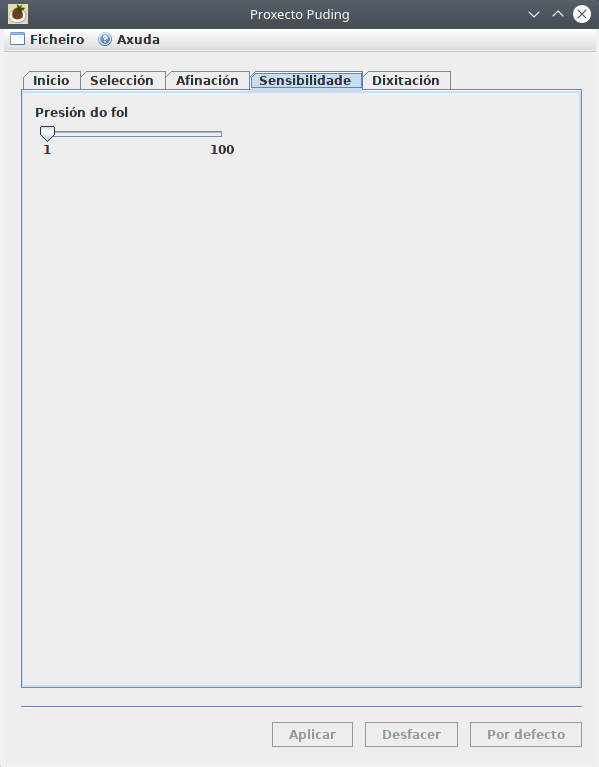
\includegraphics[scale=0.6, keepaspectratio=true]{./imagenes/configuracion-sensibilidade.png}
    % configuracion-sensibilidade.png: 640x480 pixel, 72dpi, 22.58x16.93 cm, bb=0 0 640 480
    \caption{Configuración da sensibilidade do punteiro}
    \label{figura:ConfiguracionSensibilidade}
   \end{figure}
   
   Feitos funcionar os sensores e que pasasen as probas definidas anteriormente,
   os resultados das mesmas comentaranse no apartado de probas unitarias. \\
   
   Finalmente, entre documentación, código e probas, obtivemos un módulo de moi
   baixo nivel en C de arredor de 500 liñas. \\
   
   Seguindo polo \textbf{lector de tarxetas}, a documentación proporcionada por
   4D Systems \cite{MicroDriveG1} é claramente escasa e incompleta. En xeral,
   especifica relativamente ben os casos \textit{happy path}, ou o camiño
   típico, pero en moitos casos non especifica qué pasa en caso de erro ou a
   descrición resulta ambigua, casos que cando falamos de hardware, son custosos
   cando non imposibles de reproducir de maneira forzada, o cal dificulta unha
   implementación completa e correcta do firmware. \\
   
   O proceso consistiu en:
    
   \begin{itemize}
    \item Inicializar a comunicación por porto serie.
    \item Esperar a que o dispositivo arrinque (500 ms).
    \item Esperar a que o dispositivo detecte a velocidade do porto serie.
    \item Ler ou escribir información na tarxeta de memoria.
   \end{itemize}
   
   A complexidade deste módulo residiu principalmente na incertidume na que nos
   movemos todo o rato debido á falta de documentación, que nos obrigou a estar
   probando cada pequeno paso que dabamos e a tomar decisións un pouco drásticas
   para cubrirnos en saúde. \\
   
   Basicamente, as operacións que precisamos principalmente de todas as
   dispoñibles, serían as de lectura e escritura dun ficheiro. \\
   
   Como exemplo, a documentación di que se poden ler/escribir datos en bloques
   de 1 a 50/100 bytes (con/sen ACK), pero non indica en ningún momento qué pasa
   co último bloque se o tamaño total non é múltiplo do tamaño de bloque. \\
   
   Neste caso concreto, por exemplo, optamos pola opción máis segura pero menos
   eficiente de todas: ACKs por bloques de 1 byte. Como o tamaño dos ficheiros
   é de poucos centos de bytes, a penalización apenas é perceptible. \\
   
   % TODO Revisar este punto despois de pasar as probas.
   
   Feita funcionar a lectura/escritura de ficheiros e que pasasen as probas
   definidas anteriormente, os resultados das mesmas comentaranse no apartado de
   probas unitarias. \\
   
   Finalmente, entre documentación, código e probas, obtivemos un módulo de moi
   baixo nivel en C de arredor de 700 liñas. \\
   
   E rematando polo \textbf{receptor}, que á súa vez se divide entre a lóxica
   de configuración e a de reproducción. \\
   
   Feitos funcionar os outros módulos, era o momento de implementar a lóxica de
   negocio da capa inmediatamente superior, é dicir, a do receptor, onde se
   empregrarían o módulo do lector de tarxetas para a configuración e os módulos
   de presión e capacitivos para a reproducción. \\
   
   Cabe dicir que tampouco foi tarefa fácil, dado que a documentación oficial de
   Arduino deixa moito que desexar. Conta coa información básica máis ou menos
   ben estructurada, pero en canto se quere ir un pouco máis alá, a única opción
   é consultar os foros técnicos ou aplicar o proceso de proba-erro. Moitas das
   dúbidas que se plantexan nos foros e que se ve que son bastante repetitivas
   poderían pasar a formar parte da documentación oficial coma proceso de
   mellora. \\
   
   Comezamos pola parte de reproducción, que a priori semellaba máis sinxela a
   nivel de comunicación, aínda que requería da consulta de máis sensores. \\
   
   O proceso consistiu en:
    
   \begin{itemize}
    \item Configurar o dispositivo. Cargar os módulos e mapear as dixitacións.
    \item Ler os valores dos módulos (presión e sensores capacitivos activos).
    \item Determinar se a nota e os bordóns deben soar ou non en función do
        valor do sensor de presión.
    \item Calcular a nota a reproducir en función da dixitación equivalente ós
        sensores activos.
    \item Enviar o comando MIDI correspondente para reproducir o parar nota e
        bordóns.
   \end{itemize}
   
   Para o primeiro o punto, definíronse un par de matrices que conteñen as
   dixitacións típicas da gaita galega (aberto -figura
   \ref{figura:MatrizAberto}- e pechado -figura \ref{figura:MatrizPechado}-),
   sendo a primeira parte a representación binaria equivalente dos valores
   aportados polos sensores capacitivos e a segunda o desprazamento en semitonos
   respecto da nota base ou tonalidade na que se está tocando. \\
   
   \begin{figure}[htbp]
    \centering
    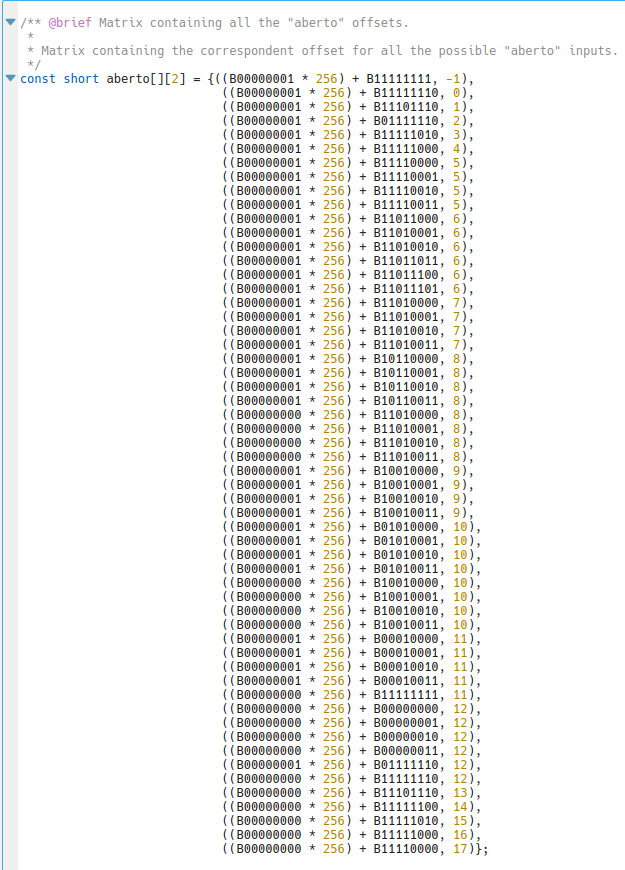
\includegraphics[scale=0.6, keepaspectratio=true]{./imagenes/matriz-aberto.png}
    % matriz-aberto.png: 640x480 pixel, 72dpi, 22.58x16.93 cm, bb=0 0 640 480
    \caption{Matriz de dixitación aberta}
    \label{figura:MatrizAberto}
   \end{figure}
   
   \begin{figure}[htbp]
    \centering
    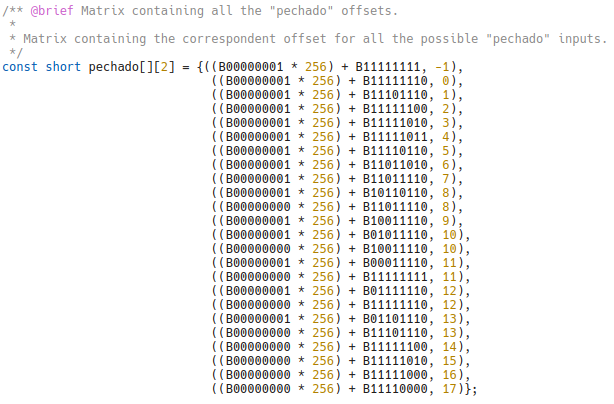
\includegraphics[scale=0.6, keepaspectratio=true]{./imagenes/matriz-pechado.png}
    % matriz-pechado.png: 640x480 pixel, 72dpi, 22.58x16.93 cm, bb=0 0 640 480
    \caption{Matriz de dixitación pechada}
    \label{figura:MatrizPechado}
   \end{figure}
   
   Para o segundo punto simplemente lemos os valores dos sensores coma durante
   as probas. \\
   
   Para determinar se deben soar ou non nota e bordóns, comparamos o valor
   obtido de presión co umbral definido como límite. Neste caso poderiamos
   incluso facer un comparador con histérese definindo un límite alto e un
   límite baixo, en función de se estamos enchendo ou baleirando o fol, pero non
   o vimos preciso. \\
   
   Para calcular a nota e os bordóns, partimos da nota base ou tonalidade e
   aplicamos o desprazamento en semitonos obtido da matriz xeral de dixitacións
   co que obtemos a nota a reproducir (no caso dos bordóns, o desprazamento é
   sempre fixo). \\
   
   Para xerar o comando MIDI a enviar ó servidor MIDI, o que fixemos foi facer
   uso dunha librería referenciada entre as da documentación de Arduino
   \ref{MIDILibrary}. Desta librería empregamos basicamente tres comandos:
   
   \begin{itemize}
    \item Note On.
    \item Note Off.
    \item Send pitch bend. Este último empregouse xunto co sensor de proximidade
        para saber cándo aplicar unha pequena variación na nota que se denomina
        vibrato.
   \end{itemize}
   
   Lista a parte de reproducción, continuamos coa parte de configuración. \\
   
   O proceso consistiu en:
    
   \begin{itemize}
    \item Ler a configuración almacenada no dispositivo xa cargado previamente.
    \item Configurar o dispositivo en función da última configuración gardada
        lida no paso anterior.
    \item Comprobar se a aplicación de configuración nos pide que nos
        identifiquemos.
    \item Comprobar se a aplicación nos solicita a configuración actual, previa
        ou por defecto e enviala no seu caso.
    \item Comprobar se a aplicación nos envía unha nova configuración.
   \end{itemize}
   
   Para o intercambio e almacenamento da configuración precisábase un formato
   lixeiro pero ó mesmo tempo facilmente lexible e modificable, polo que se
   optou por empregar JSON. \\
   
   O tratamento de JSON en Arduino está todavía un pouco verde. No momento no
   que se avaliou a dispoñibilidade de librerías para o seu tratamento a máis
   coñecida era \textit{aJSON} \cite{aJSON} cuxo desenvolvemento parece morto
   a día de hoxe e que aínda conta con decenas de incidencias abertas. \\
   
   Actualmente, a máis empregada aínda que tamén con decenas de incidencias
   abertas é \textit{Arduino Json} \cite{ArduinoJson}. Pero como a
   implementación se fixo antes de que isto ocorrese, empregouse aJSON. \\
   
   Como xa comentamos anteriormente, cada dispositivo garda a súa propia
   configuración. A nivel de implementación, garda un ficheiro por cada tipo de
   configuración (selección, sensibilidade, etc.) e de acción (actual, previa ou
   por defecto), de maneira que cada dispositivo conta con máis dunha ducia de
   pequenos ficheiros de configuración almacenados. \\
   
   Cada un deses ficheiros de configuración non é máis ca un ficheiro de texto
   plano que contén unha tipo de configuración en formato JSON (figura
   \ref{figura:FicheiroJson}). \\
   
   \begin{figure}[htbp]
    \centering
    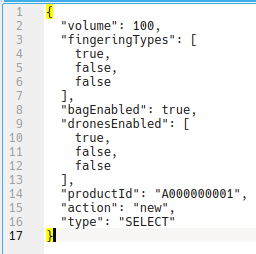
\includegraphics[scale=0.6, keepaspectratio=true]{./imagenes/ficheiro-json.png}
    % ficheiro-json.png: 640x480 pixel, 72dpi, 22.58x16.93 cm, bb=0 0 640 480
    \caption{Ficheiro de configuración en formato JSON}
    \label{figura:FicheiroJson}
   \end{figure}
   
   Os fluxos de identificación e configuración comentaranse na parte software,
   xa que é máis doado entendelos relacionándoos coa interación do usuario sobre
   as pantallas. \\
   
   Finalmente, entre documentación e código, obtivemos un módulo de baixo nivel
   en C de arredor de 1100 liñas. \\
   
   Sen embargo, á hora de querer cargar o código na placa atopámonos con
   problemas, que explicaremos no apartado de indicencias, e que fixeron que
   tiveramos que, logo de aplicar o análise de riscos e alternativas, optaramos
   por empregar unha versión simplificada, de arredor de 700 liñas. \\
   
   As probas de integración da parte hardware leváronse a cabo xunto coa parte
   software, motivo polo que se postergan os resultados obtidos ata a
   finalización da aplicación de configuración que, ademáis de xestionar a mesma
   é a encargada de levantar o servidor MIDI cos parámetros correctos.
   
   \paragraph{Software}
   
   Lista a implementación da parte hardware, tocoulle o turno á parte
   software. \\
   
   En xeral, para toda a implementación e as probas da aplicación empregouse
   (ou está en trámites de actualizarse pouco a pouco) inxección de dependencias
   (mediante \textit{Guice} \ref{Guice}), obxectos inmutables (mediante
   \textit{Guava} \ref{Guava}) e programación funcional (mediante expresións
   lambda de Java 8). \\
   
   Se lembramos dos apartados anteriores, tiñamos pendente a implementación da
   capa de servizos hacia abaixo. Concretamente:
   
   \begin{itemize}
    \item O servizo de dispositivos.
    \item O servizo de configuración.
    \item O servizo de internacionalización.
    \item O servizo de notificacións.
    \item O servizo de navegación web.
    \item E o servizo MIDI.
   \end{itemize}
   
   O \textbf{servizo de dispositivos} é o encargado de xestionar todo o
   relacionado cos dispositivos hardware en uso: detección, comunicación,
   etc. \\
   
   Para poder comunicarnos cos dispositivos a través do router XBee, que se
   conecta ó ordenador mediante USB, precisabamos dunha librería de comunicación
   serie para Java. \\
   
   A base de buscar e de falar con xente do mundillo, demos coa librería RXTX de
   GNU \cite{RXTX}, ó parecer, a única dispoñible daquelas e constatamos que a
   comunicación serie é un dos grandes olvidados en Java. \\
   
   A instalación da mesma foi farragosa e o seu uso infructuoso, pois non fomos
   quen de conseguir conectividade, polo cal a implementación final quedou en
   espera a falta de alternativas. \\
   
   Finalmente, uns anos despois, apareceu unha nova librería,
   \textit{Java Simple Serial Connector} ou \textit{jSSC} \cite{jSSC} que, lonxe
   de ser perfecta, ofrece menos dificultades tanto para a súa instalación coma
   para o seu uso. En todo caso, leva parada hai moitos anos. \\
   
   Ademáis da librería de comunicación serie, era precisa unha librería para o
   tratamento de JSON, pois era o formato a empregar durante as
   comunicacións. \\
   
   Neste caso, a elección estivo bastante clara dende un principio. A librería 
   \textit{Gson} \cite{Gson} foi a escollida, por ser amplamente empregada no
   mundo Java. \\
   
   Tendo claras xa as librerías, a outra parte interesante é o fluxo de datos
   entre a aplicación e os dispositivos. Concretamente para os casos de:
   
   \begin{itemize}
    \item Detección de dispositivos.
    \item Recuperación da configuración dun dispositivo.
    \item Envío dunha nova configuración a un dispositivo.
   \end{itemize}
   
   Os diagramas de fluxo dos casos anteriores poden apreciarse nas figuras
   \ref{figura:DeteccionDispositivos} a \ref{EnvioConfiguracion}. \\
   
   \begin{figure}[htbp]
    \centering
    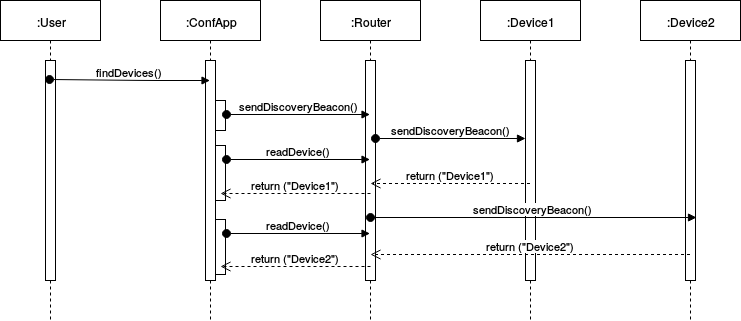
\includegraphics[scale=0.5, keepaspectratio=true]{./imagenes/df-find-devices.png}
    % df-find-devices.png: 640x480 pixel, 72dpi, 22.58x16.93 cm, bb=0 0 640 480
    \caption{Detección de dispositivos}
    \label{figura:DeteccionDispositivos}
   \end{figure}
   
   \begin{figure}[htbp]
    \centering
    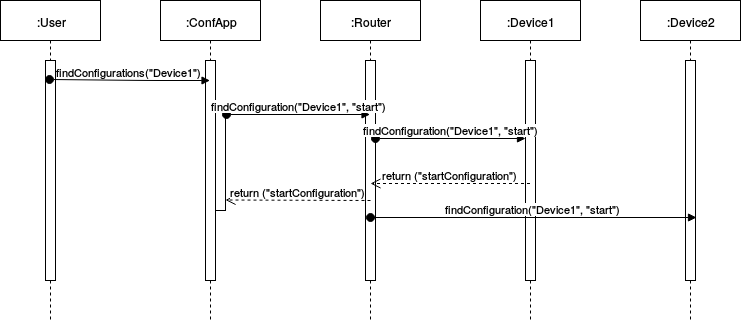
\includegraphics[scale=0.5, keepaspectratio=true]{./imagenes/df-select-device.png}
    % df-select-device.png: 640x480 pixel, 72dpi, 22.58x16.93 cm, bb=0 0 640 480
    \caption{Recuperación da configuración dun dispositivo}
    \label{figura:RecuperacionConfiguracion}
   \end{figure}
   
   \begin{figure}[htbp]
    \centering
    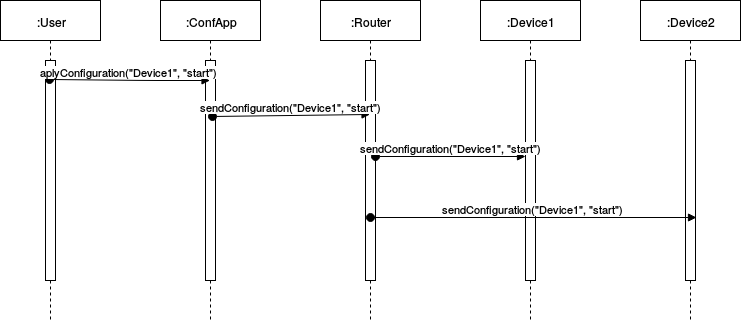
\includegraphics[scale=0.5, keepaspectratio=true]{./imagenes/df-apply-config.png}
    % df-apply-config.png: 640x480 pixel, 72dpi, 22.58x16.93 cm, bb=0 0 640 480
    \caption{Envío dunha nova configuración a un dispositivo}
    \label{figura:EnvioConfiguracion}
   \end{figure}
   
   No diagrama de detección de dispositivos (figura
   \ref{figura:DeteccionDispositivos}) podemos apreciar como cando o usuario
   busca dispositivos se envía unha baliza de recoñecemento que chega a todos
   os dispositivos conectados ó router mediante broadcasting. Dita baliza indica
   ós dispostivos que deben identificarse. \\
   
   Unha vez identificados pola aplicación e seleccionado un deles polo usuario,
   recupérase a configuración do mesmo, indicando na petición o identificador do
   dispositivo, que queremos a configuración actual e o tipo en cada caso
   (figura \ref{figura:RecuperacionConfiguracion}). \\
   
   Cando o usuario precise axustar algún parámetro, enviará a nova configuración
   ó dispositivo, indicando na petición o identificador do dispositivo, que é
   unha nova configuración e o tipo en cada caso, que acto seguido será aplicada
   polo dispositivo, segundo se amosa na figura
   \ref{figura:EnvioConfiguracion}. \\
   
   O \textbf{servizo de configuración} é o encargado de xestionar todo o
   relacionado coa configuración da aplicación, servindo de ponte entre esta e
   outros servizos coma o de dispositivos ou o MIDI. \\
   
   Encárgase de cousas como de precargar os datos de configuración dos menús
   da aplicación ou de xerar a configuración do servidor MIDI en función dos
   valores da configuración actual. \\
   
   En canto á precarga dos datos de configuración dos menús da aplicación, a
   dificultade estribaba en que é dependente da tonalidade de lectura do usuario
   polo que para as mesmas claves/notas, temos valores/nomes distintos en
   función da tonalidade na que o usuario teña configurada a aplicación. \\
   
   A xeración da configuración para o servidor MIDI non reviste máis
   complexidade que a de facer un mapeo dos valores da configuración dos que
   depende o mesmo para funcionar o máis precisamente posible (figura
   \ref{figura:MapeoConfiguracionServidorMIDI}). \\
   
   \begin{figure}[htbp]
    \centering
    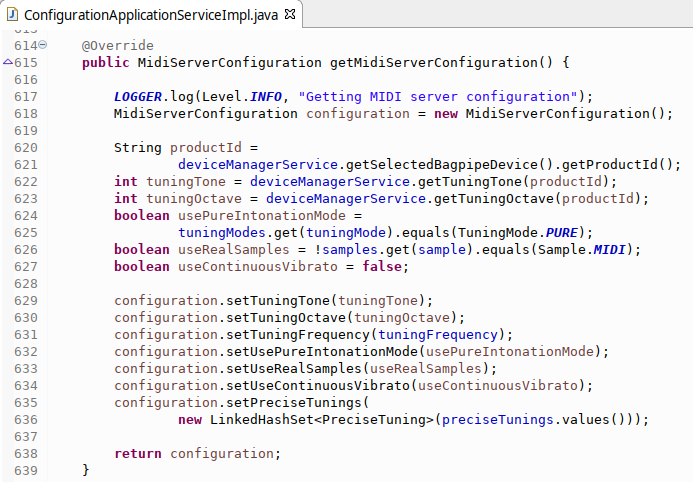
\includegraphics[scale=0.6, keepaspectratio=true]{./imagenes/mapeo-conf-servidor-midi.png}
    % mapeo-conf-servidor-midi.png: 640x480 pixel, 72dpi, 22.58x16.93 cm, bb=0 0 640 480
    \caption{Mapeo da configuración do servidor MIDI}
    \label{figura:MapeoConfiguracionServidorMIDI}
   \end{figure}
   
   O \textbf{servizo de internacionalización} é o encargado de proporcionar as
   mensaxes da aplicación no idioma do usuario. \\
   
   Actualmente adopta o idioma do sistema e conta con soporte para galego e
   inglés (por defecto). \\
   
   O \textbf{servizo de notificacións}, encargado de xestionar a comunciación
   entre as distintas partes da interface mediante eventos. \\
   
   Basicamente trátase dun patrón observador cun conxunto de notificacións
   predefinidas (figura \ref{figura:Notificacions}) ás que se pode subscribir
   calquera compoñente da aplicación que o precise. \\
   
   \begin{figure}[htbp]
    \centering
    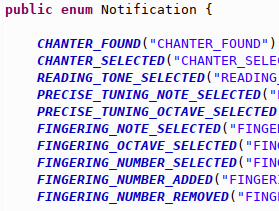
\includegraphics[scale=0.6, keepaspectratio=true]{./imagenes/notificacions.png}
    % notificacions.png: 640x480 pixel, 72dpi, 22.58x16.93 cm, bb=0 0 640 480
    \caption{Notificacións}
    \label{figura:Notificacions}
   \end{figure}
   
   Resulta moi útil e simplifica enormemente a actualización de valores entre
   pestanas da aplicación. \\
   
   O \textbf{servizo de navegación web}, xestiona a apertura da documentación da
   aplicación (web do proxecto, manual de usuario, APIs, etc.) directamente no
   navegador do sistema (figura \ref{figura:Navegador}). \\
   
   \begin{figure}[htbp]
    \centering
    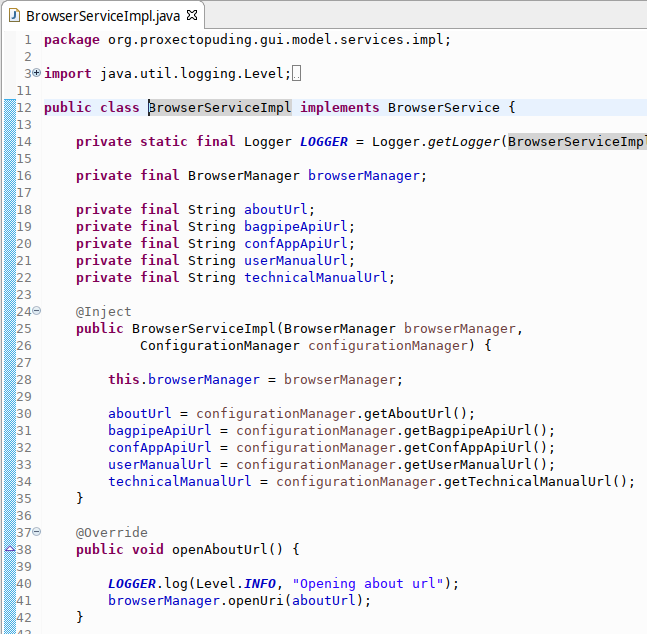
\includegraphics[scale=0.6, keepaspectratio=true]{./imagenes/navegador.png}
    % navegador.png: 640x480 pixel, 72dpi, 22.58x16.93 cm, bb=0 0 640 480
    \caption{Servizo de navegación web}
    \label{figura:Navegador}
   \end{figure}
   
   O \textbf{servizo MIDI}, xestiona todo o relacionado coas operacións sobre o
   servidor MIDI: configurar, levantar e parar o servidor. \\
   
   Neste caso, o que se buscou foi contar cunha representación única xenérica do
   servidor MIDI e da súa configuración que logo se particularizou segundo o
   sistema operativo anfitrión e o servidor MIDI particular mediante o uso dun
   patrón estratexia. \\
   
   Para o servidor MIDI, aínda que poderiamos ter aplicado un distinto para cada
   sistema operativo, optamos por buscar e empregar o mesmo para todos, de ser
   posible, particularizando logo o comando de execución para cada sistema
   operativo segundo o caso. \\
   
   A opción escollida foi \textbf{Timidity} \cite{Timidity}, un sintetizador
   MIDI de amplo uso e con soporte para gran cantidade de sistemas
   operativos. \\
   
   Como alternativa dispoñemos de FluidSynth \cite{FluidSynth}, máis moderno,
   pero con menos funcionalidades relacionadas co proxecto ca Timidity, motivo
   polo que apostamos por este último. \\
   
   Timidity conta con soporte para uso de fontes de son alternativas (son real),
   táboas de frecuencias personalizadas (afinación natural e axuste fino por
   nota), vibrato continuo, etc., tal e como se pode comprobar na figura
   \ref{figura:Timidity}. \\
   
   \begin{figure}[htbp]
    \centering
    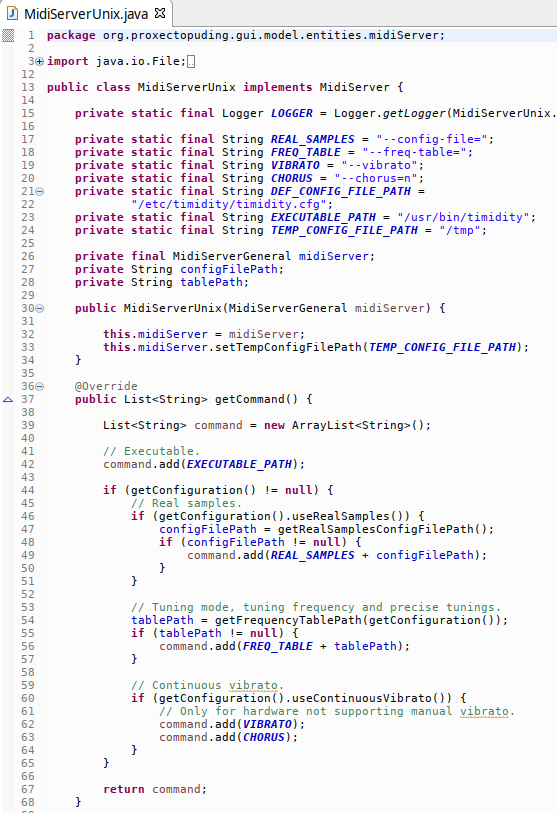
\includegraphics[scale=0.6, keepaspectratio=true]{./imagenes/timidity.png}
    % timidity.png: 640x480 pixel, 72dpi, 22.58x16.93 cm, bb=0 0 640 480
    \caption{Servizo MIDI: sistemas UNIX}
    \label{figura:Timidity}
   \end{figure}
   
   Como partes interesantes desta implementación, destacar por unha banda o
   xestor de descargas de fontes de son, dado que para fontes de son realistas
   o peso é demasiado elevado como para almacenala no propio repositorio da
   aplicación e, ademáis, gañamos poder manter actualizada a fonte de son en
   todos os clientes. \\
   
   Tamén é destacable o cálculo da táboa de frecuencias para afinación natural.
   É teoría musical, pero que precisamos plasmar na nosa implementación de
   maneira programática. \\
   
   A nivel código non deixa de ser unha relación matemática entre a tonalidade
   base e o resto da súa escala musical. \\
   
   No caso dunha escala temperada, estas relacións as mesmas para toda a escala,
   é dicir, se un tono se divide en 9 comas, os semitonos están equiespaciados a
   razón de 4,5 comas por semitono \cite{AfinacionTemperada}. \\
   
   No caso dunha escala natural (tamén chamada xusta ou pura), os semitonos
   están espaciados a razón de 4 ou 5 comas segundo o caso
   \cite{AfinacionNatural}. \\
   
   Isto fai que os harmónicos (ou frecuencias harmónicas) producidos por cada
   nota varíen moito dun tipo de escala ó outro e, polo tanto, a mesma escala
   reproducida cunha afinación ou a outra soe de maneira moi distinta. \\
   
   Dentro da propia afinación xusta, existen moitas variantes xa dende os tempos
   de Pitágoras pero, en xeral, o que se busca é obter o maior número de tríadas
   posibles que xeren intervalos consonantes, é dicir, que os harmónicos ou
   frecuencias harmónicas xerados polas tres notas do acorde ou tríada, sexan
   consonantes entre si \cite{Escalas}. \\
   
   As relacións máis empregadas para a afinación xusta son as da figura
   \ref{figura:AfinacionNatural}. \\
   
   \begin{figure}[htbp]
    \centering
    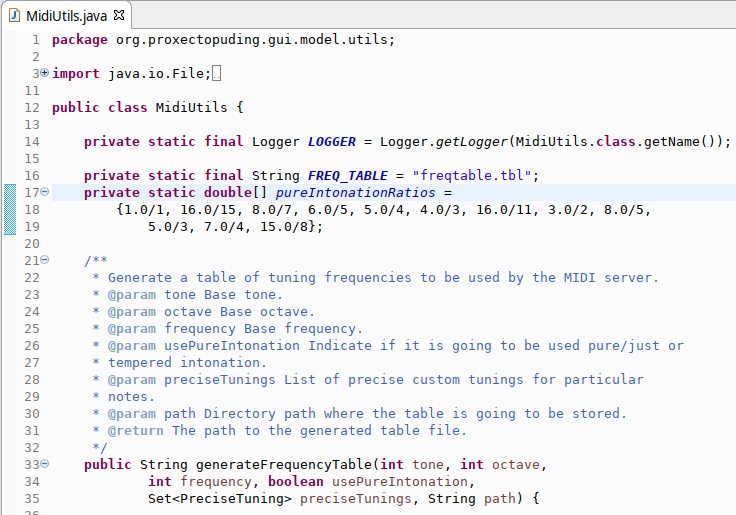
\includegraphics[scale=0.6, keepaspectratio=true]{./imagenes/afinacion-natural.png}
    % afinacion-natural.png: 640x480 pixel, 72dpi, 22.58x16.93 cm, bb=0 0 640 480
    \caption{Relacións afinación xusta}
    \label{figura:AfinacionNatural}
   \end{figure}
   
   Finalmente, entre documentación, código (de alto, medio e baixo nivel) e
   probas (de unidade, integración e aceptación), obtivemos unha aplicación de
   arredor de 15000 liñas de código en Java. \\
   
   A parte de probas será reflexada con detalle na sección correspondente.
   
 \subsection{Probas de unidade}
 
 Seguindo os principios de TDD, as probas de unidade foron paso previo á
 implementación real tanto dos módulos hardware coma dos servizos sofware.
 
  \subsubsection{Hardware}
  
  % TODO Revisar toda esta sección hardware.
  
  Como comentamos anteriormente, durante o desenvolvemento do prototipo hardware
  operacional creáronse uns pequenos sketches de exemplo a modo de probas
  unitarias, para poder validar o funcionamento de cada módulo por separado
  antes de proceder á súa integración na montaxe do receptor. \\
  
  No caso do sensor de presión, probamos a obtención da temperatura e presión
  ambiente, aínda que para o caso que nos ocupa, con probar a presión sería
  suficiente (figura \ref{figura:TestUnitarioSensorPresion}). \\
  
  \begin{figure}[htbp]
   \centering
   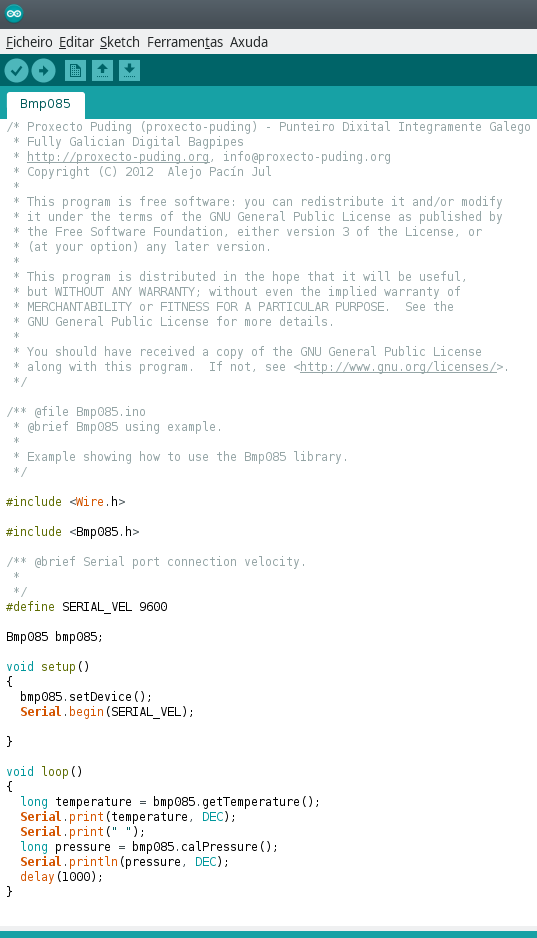
\includegraphics[scale=0.8,keepaspectratio=true]{./imagenes/test-sensor-presion.png}
   % test-sensor-presion.png: 640x480 pixel, 72dpi, 22.58x16.93 cm, bb=0 0 640 480
   \caption{Probas de unidade do sensor de presión}
   \label{figura:TestUnitarioSensorPresion}
  \end{figure}
  
  Os resultados obtidos pódense ver na figura
  \ref{figura:ResultadoTestUnitarioSensorPresion}. Salientar que arroxa uns
  valores algo altos froito de que está calibrado para obter o resultado o máis
  rápido posible, reducindo polo tanto a precisión ó mínimo. Pero como o que
  precisamos é básicamente un valor para comparar con un umbral, é perfectamente
  válido. \\
  
  \begin{figure}[htbp]
   \centering
   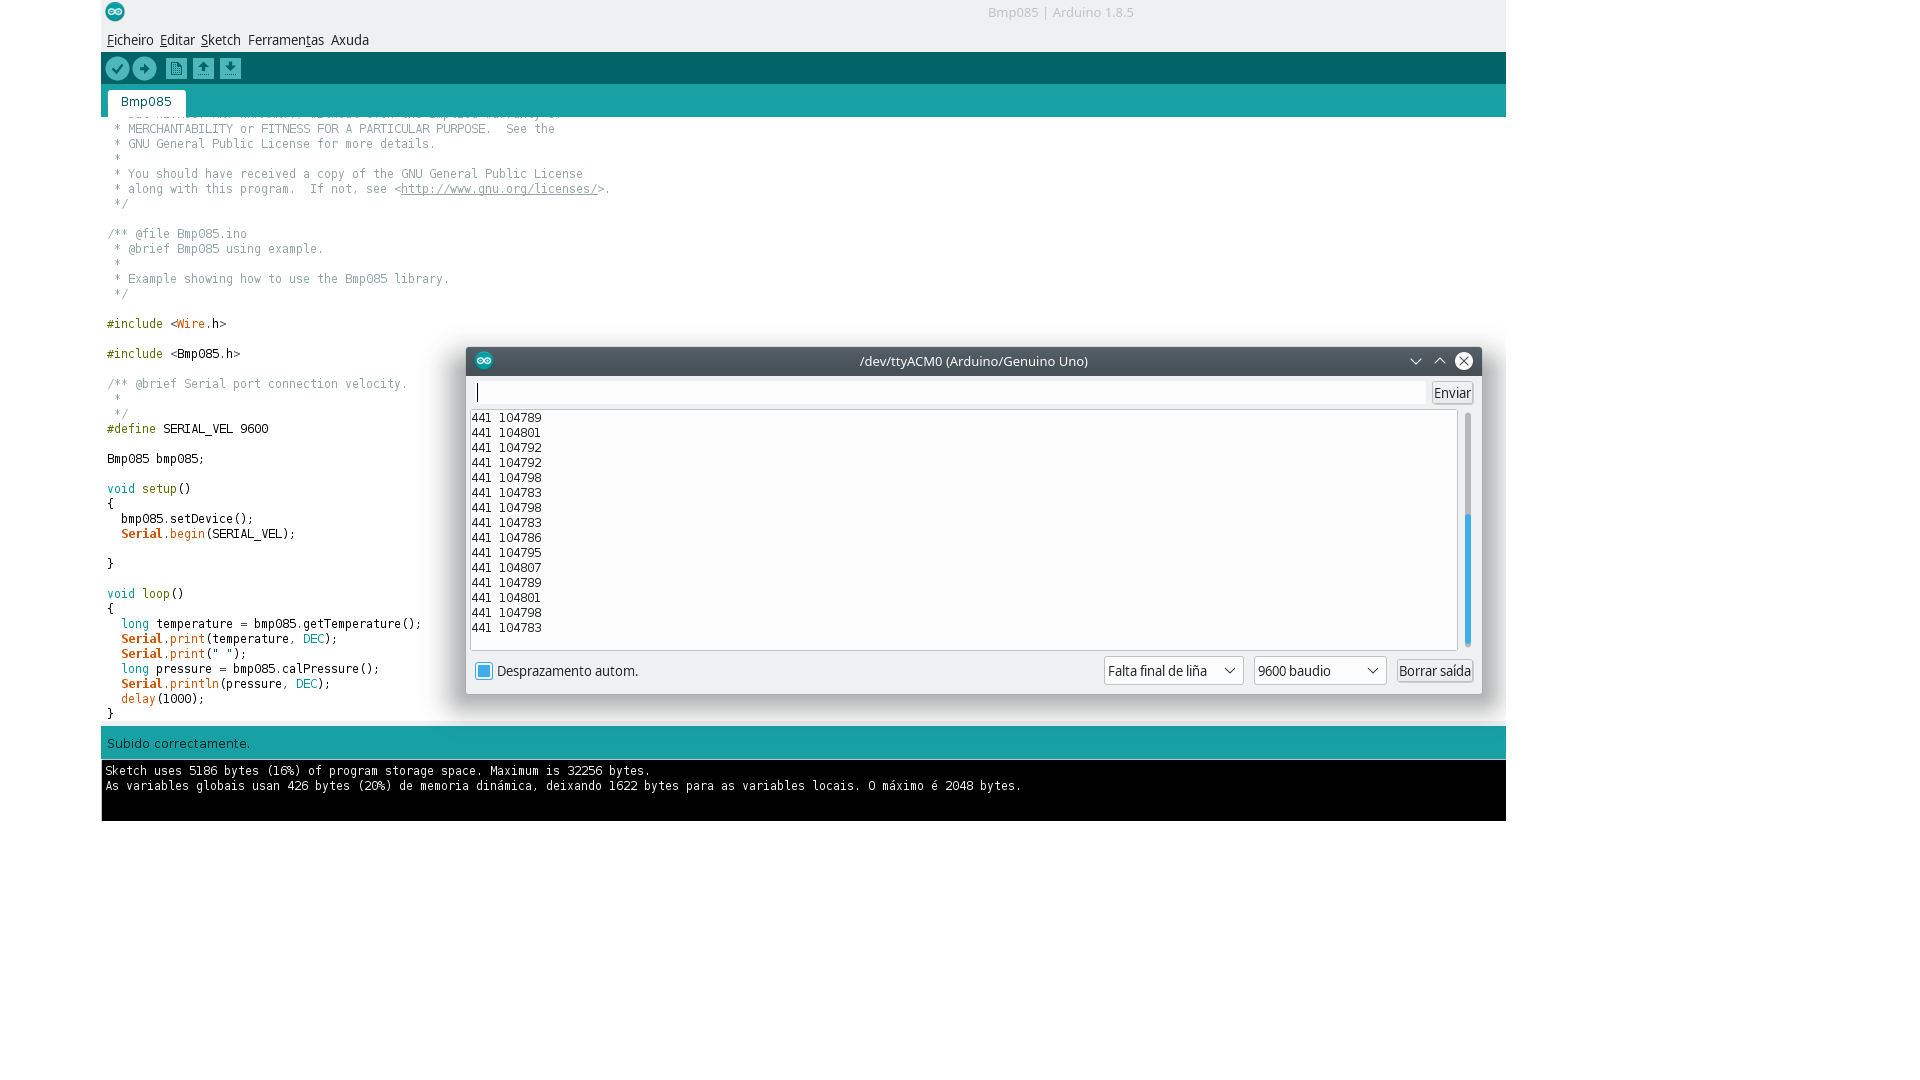
\includegraphics[scale=0.8,keepaspectratio=true]{./imagenes/resultado-test-sensor-presion.png}
   % resultado-test-sensor-presion.png: 640x480 pixel, 72dpi, 22.58x16.93 cm, bb=0 0 640 480
   \caption{Resultado das probas de unidade do sensor de presión}
   \label{figura:ResultadoTestUnitarioSensorPresion}
  \end{figure}
  
  No caso dos sensores capacitivos, probamos a ler os valores dos nove bits
  menos significativos máis o bit do sensor de proximidade. Neste caso, a
  entrada é manual e precisa da intervención do usuario, que debe validar
  visualmente que o resultado obtivo se corresponde coa entrada manual
  (figura \ref{figura:TestUnitarioSensoresCapacitivos}).
   
  \begin{figure}[htbp]
   \centering
   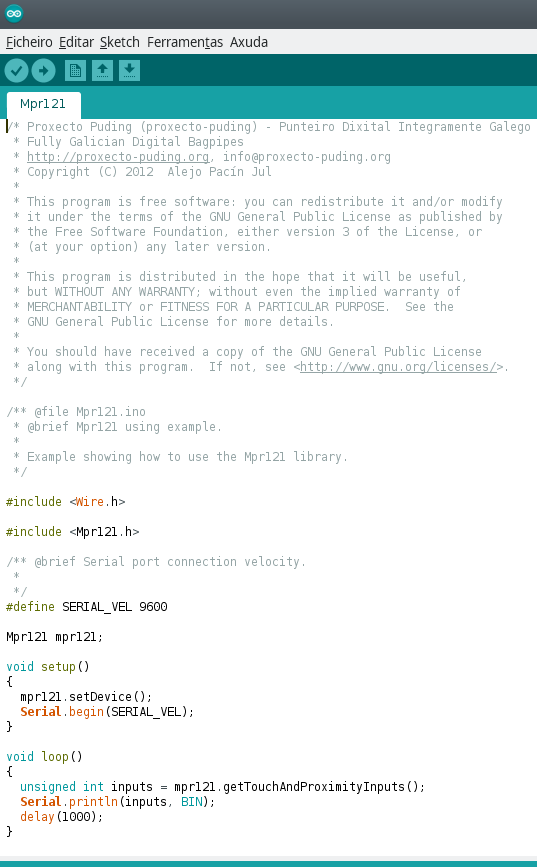
\includegraphics[scale=0.8,keepaspectratio=true]{./imagenes/test-sensores-capacitivos.png}
   % test-sensores-capacitivos.png: 640x480 pixel, 72dpi, 22.58x16.93 cm, bb=0 0 640 480
   \caption{Probas de unidade dos sensores capacitivos}
   \label{figura:TestUnitarioSensoresCapacitivos}
  \end{figure}
  
  Os resultados obtidos pódense ver na figura
  \ref{figura:ResultadoTestUnitarioSensoresCapacitivos}. Validados os resultados
  de forma visual, comprobouse que eran correctos. \\
  
  \begin{figure}[htbp]
   \centering
   \includegraphics[scale=0.8,keepaspectratio=true]{./imagenes/resultado-test-sensores-capacitivos.png}
   % resultado-test-sensores-capacitivos.png: 640x480 pixel, 72dpi, 22.58x16.93 cm, bb=0 0 640 480
   \caption{Resultado das probas de unidade dos sensores capacitivos}
   \label{figura:ResultadoTestUnitarioSensoresCapacitivos}
  \end{figure}
  
  No caso do lector de tarxetas, probamos a ler a información do dispositivo,
  listar o directorio principal, escribir, mover e ler un ficheiro. Aínda que
  con probar a ler e escribir sería suficiente para cubrir as nosas necesidades
  (figura \ref{figura:TestUnitarioLectorTarxetas}). \\
  
  \begin{figure}[htbp]
   \centering
   \includegraphics[scale=0.8,keepaspectratio=true]{./imagenes/test-lector-tarxetas.png}
   % test-lector-tarxetas.png: 640x480 pixel, 72dpi, 22.58x16.93 cm, bb=0 0 640 480
   \caption{Ficheiro de proba do lector de tarxetas}
   \label{figura:TestUnitarioLectorTarxetas}
  \end{figure}
  
  Os resultados obtidos pódense ver na figura
  \ref{figura:ResultadoTestUnitarioLectorTarxetas}. Validados os resultados
  de forma visual e revisada externamente a tarxeta de memoria, comprobouse que
  eran correctos. \\
  
  \begin{figure}[htbp]
   \centering
   \includegraphics[scale=0.8,keepaspectratio=true]{./imagenes/resultado-test-lector-tarxetas.png}
   % resultado-test-lector-tarxetas.png: 640x480 pixel, 72dpi, 22.58x16.93 cm, bb=0 0 640 480
   \caption{Ficheiro de proba do lector de tarxetas}
   \label{figura:ResultadoTestUnitarioLectorTarxetas}
  \end{figure}
  
  \subsubsection{Software}
  
  Como comentamos tamén anteriormente, durante o desenvolvemento do prototipo
  software operacional creáronse baterías de tests unitarios a nivel de
  servizo. \\
  
  Creouse unha batería de tests por servizo (figura \ref{figura:TestsUnitarios}
  e cubriuse alomenos o \textit{happy path} de cada unha das súas sinaturas. \\
  
  \begin{figure}[htbp]
   \centering
   \includegraphics[scale=0.8,keepaspectratio=true]{./imagenes/tests-unitarios.png}
   % test-unitarios.png: 640x480 pixel, 72dpi, 22.58x16.93 cm, bb=0 0 640 480
   \caption{Tests unitarios}
   \label{figura:TestUnitarios}
  \end{figure}
  
  Para simular o comportamento de cada método empregouse unha librería de
  \textit{mocking}. A escollida, pola súa popularidade dentro do mundo Java foi
  \textit{Mockito} \cite{Mockito}. \\
  
  \begin{figure}[htbp]
   \centering
   \includegraphics[scale=0.8,keepaspectratio=true]{./imagenes/test-mockito.png}
   % test-mockito.png: 640x480 pixel, 72dpi, 22.58x16.93 cm, bb=0 0 640 480
   \caption{Exemplo de test unitario con Mockito}
   \label{figura:TestMockito}
  \end{figure}
  
  Vexamos un exemplo. Como se pode apreciar na figura \ref{figura:TestMockito},
  nas precondicións configuráse o comportamento do mock. Logo execútase a
  operación que se quere probar e finalmente compróbanse as poscondicións. \\
  
  É de salientar que, aínda que máis propio de BDD, intentou empregarse linguaxe
  \textit{Gherkin} \cite{Gherkin} tanto como foi posible para que os tests fóran
  o máis sinxelos de ler posible. \\
  
  \begin{figure}[htbp]
   \centering
   \includegraphics[scale=0.8,keepaspectratio=true]{./imagenes/resultados-tests-unitarios.png}
   % resultados-test-unitarios.png: 640x480 pixel, 72dpi, 22.58x16.93 cm, bb=0 0 640 480
   \caption{Resultados tests unitarios}
   \label{figura:ResultadosTestUnitarios}
  \end{figure}
  
  Executadas as probas, cun total de 48 tests unitarios, podemos comprobar que
  todas pasan correctamente (figura \ref{figura:ResultadosTestUnitarios}).

 \subsection{Integración e probas}
 
 Durante o desenvolvemento do prototipo software operacional creáronse baterías
 de tests de integración a nivel de servizo. \\
 
 Creouse unha batería de tests por servizo (figura \ref{figura:TestsIntegracion}
 e cubriuse alomenos o \textit{happy path} de cada unha das súas sinaturas. \\
  
  \begin{figure}[htbp]
   \centering
   \includegraphics[scale=0.8,keepaspectratio=true]{./imagenes/tests-integracion.png}
   % test-integracion.png: 640x480 pixel, 72dpi, 22.58x16.93 cm, bb=0 0 640 480
   \caption{Tests de integración}
   \label{figura:TestsIntegracion}
  \end{figure}
  
  Vexamos un exemplo. Como se pode apreciar na figura \ref{figura:TestIntegracion},
  créanse as precondicións, logo execútase a operación que se quere probar e
  finalmente compróbanse as poscondicións. \\
  
  \begin{figure}[htbp]
   \centering
   \includegraphics[scale=0.8,keepaspectratio=true]{./imagenes/test-integracion.png}
   % test-integracion.png: 640x480 pixel, 72dpi, 22.58x16.93 cm, bb=0 0 640 480
   \caption{Exemplo de test de integración}
   \label{figura:TestIntegracion}
  \end{figure}
  
  É de salientar que, aínda que máis propio de BDD, intentou empregarse linguaxe
  \textit{Gherkin} \cite{Gherkin} tanto como foi posible para que os tests fóran
  o máis sinxelos de ler posible. \\
 
 Aquí a aproximación consistiu en executar os tests tendo o hardware conectado ó
 pc executando a aplicación. \\
 
 \begin{figure}[htbp]
  \centering
  \includegraphics[scale=0.6,keepaspectratio=true]{./imagenes/resultados-tests-integracion.png}
  % resultados-test-integracion.png: 640x480 pixel, 72dpi, 22.58x16.93 cm, bb=0 0 640 480
  \caption{Resultados tests integracion}
  \label{figura:ResultadosTestIntegracion}
 \end{figure}
  
 Executadas as probas, cun total de 133 tests de integración, podemos comprobar
 que non todas pasan correctamente
 (figura \ref{figura:ResultadosTestIntegracion}). \\
 
 Concretamente, se nos fixamos en ditos resultados, as que non pasan son as
 que precisan conectividade co dispositivo. Isto débese a unha incidencia que se
 deu durante o desenvolvemento e que xa comentamos anteriormente, que nos levou
 a ter que empregar unha versión simplificada do firmware do dispositivo. Dita
 incidencia detallarase na sección correspondente. \\
 
 Para as suites de tests que fallan, para intentar paliar este problema,
 desenvolvéronse uns tests de integración alternativos (co sufixo Mock), no que
 se simula o intercambio de información en formato JSON co dispositivo, de
 maneira que alomenos poidamos verificar e validar a aplicación de configuración
 incluíndo a serialización e deserialización da información, tal e como se faría
 cun dispositivo real. É dicir, contamos cun dispositivo simulado en Java que
 emite e recibe información en formato JSON, tal coma o identificador ou os
 distintos tipos de configuración. \\
 
 \begin{figure}[htbp]
  \centering
  \includegraphics[scale=0.8,keepaspectratio=true]{./imagenes/tests-integracion-conectividade.png}
  % tests-integracion-conectividade.png: 640x480 pixel, 72dpi, 22.58x16.93 cm, bb=0 0 640 480
  \caption{Tests de integración da conectividade}
  \label{figura:TestsIntegracionConectividade}
 \end{figure}
  
 Así mesmo, para probar que a conectividade co dispositivo funciona e polo
 tanto a librería serie en Java cumpría co seu cometido (dado que coa primeira
 escollida tamén tivemos problemas), desenvolvéronse un par de tests extra de
 integración da conectividade e os seus sketches asociados (figura
 \ref{figura:TestsIntegracionConectividade}). \\
  
 \begin{figure}[htbp]
  \centering
  \includegraphics[scale=0.8,keepaspectratio=true]{./imagenes/test-integracion-conectividade.png}
  % test-integracion-conectividade.png: 640x480 pixel, 72dpi, 22.58x16.93 cm, bb=0 0 640 480
  \caption{Tests de integración da conectividade}
  \label{figura:TestIntegracionConectividade}
 \end{figure}
 
 Na figura \ref{figura:TestIntegracionConectividade} podemos apreciar o segundo
 dos mesmos e o máis complexo, que trata de xogar ó ping-pong cunha cadea de
 texto entre a aplicación e o dispositivo. \\
 
 \begin{figure}[htbp]
  \centering
  \includegraphics[scale=0.45,angle=90,keepaspectratio=true]{./imagenes/resultados-tests-integracion-conectividade.png}
  % resultados-tests-integracion-conectividade.png: 640x480 pixel, 72dpi, 22.58x16.93 cm, bb=0 0 640 480
  \caption{Resultados dos tests de integración da conectividade}
  \label{figura:ResultadosTestsIntegracionConectividade}
 \end{figure}
 
 Tal e como se pode comprobar na figura
 \ref{figura:ResultadosTestsIntegracionConectividade}, as probas pasaron
 correctamente. \\
 
 Executadas as probas, cun total de 135 tests de integración, puidemos validar a
 aplicación de configuración e a conectividade co dispositivo hardware.
 
 \subsection{Probas de aceptación}
 
 Durante o desenvolvemento do prototipo software operacional creáronse baterías
 de tests de aceptación a nivel de servizo. \\
 
 Creouse unha batería de tests por servizo (figura \ref{figura:TestsIntegracion}
 e cubriuse alomenos o \textit{happy path} de cada unha das súas sinaturas. \\
  
 \begin{figure}[htbp]
  \centering
  \includegraphics[scale=0.8,keepaspectratio=true]{./imagenes/tests-aceptacion.png}
  % test-aceptacion.png: 640x480 pixel, 72dpi, 22.58x16.93 cm, bb=0 0 640 480
  \caption{Tests de aceptación}
  \label{figura:TestsAceptacion}
 \end{figure}
 
 As probas de aceptación fixéronse en todo momento seguindo os principios de
 BDD, deseñando os tests en base á interacción do usuario coa aplicación e
 especificando os mesmos empregando linguaxe Gherkin. \\
 
 Vexamos un exemplo. Como se pode apreciar na figura \ref{figura:TestAceptacion},
 créanse as precondicións, logo execútase a operación que se quere probar e
 finalmente compróbanse as poscondicións. \\
 
 Se nos fixamos na documentación da suite e do test, vemos como están
 especificados en linguaxe Gherkin, onde a suite é proba unha funcionalidade
 onde se poden dar varios escenarios, que é o que se describe e proba nos
 tests. \\
 
 Desta maneira, os propios tests de aceptación poden servir de contrato entre
 partes, xa que os requisitos se poden especificar en base a funcionalidades con
 distintos escenarios e, se os tests de aceptación pasan, cúmprese co
 contrato asinado. \\
  
 \begin{figure}[htbp]
  \centering
  \includegraphics[scale=0.8,keepaspectratio=true]{./imagenes/test-aceptacion.png}
  % test-aceptacion.png: 640x480 pixel, 72dpi, 22.58x16.93 cm, bb=0 0 640 480
  \caption{Exemplo de test de aceptación}
  \label{figura:TestAceptacion}
 \end{figure}
 
 A aproximación dos tests de aceptación foi a mesma que a dos de integración,
 tendo o hardware conectado ó pc executando a aplicación. \\
 
 \begin{figure}[htbp]
  \centering
  \includegraphics[scale=0.6,keepaspectratio=true]{./imagenes/resultados-tests-aceptacion.png}
  % resultados-test-aceptacion.png: 640x480 pixel, 72dpi, 22.58x16.93 cm, bb=0 0 640 480
  \caption{Resultados tests aceptación}
  \label{figura:ResultadosTestAceptacion}
 \end{figure}
  
 Executadas as probas, cun total de 11 tests de aceptación, podemos comprobar
 que non todas pasan correctamente
 (figura \ref{figura:ResultadosTestAceptacion}). \\
 
 Concretamente, se nos fixamos en ditos resultados, as que non pasan son, ó
 igual que no caso dos tests de integración, as que precisan conectividade co
 dispositivo, polo mesmo motivo. \\
 
 Para as suites de tests que fallan, para intentar paliar este problema,
 desenvolvéronse uns tests de aceptación alternativos (co sufixo Mock), no que
 se simula o intercambio de información en formato JSON co dispositivo, de
 maneira que alomenos poidamos verificar e validar a aplicación de configuración
 incluíndo a serialización e deserialización da información, tal e como se faría
 cun dispositivo real. É dicir, contamos cun dispositivo simulado en Java que
 emite e recibe información en formato JSON, tal coma o identificador ou os
 distintos tipos de configuración. \\
 
 Ademáis de todo o anterior, examinando a interacción do usuario coa interface
 para documentar os casos de proba, démonos conta de que no caso de que a busca
 dos dispositivos fallase, o usuario non tiña maneira de reintentar dita busca
 máis que pechando e volvendo abrir a aplicación, o que desde o punto de vista
 de UX non ten sentido, polo que se procedeu a incluír un botón de busca na
 pantalla de inicio (figura \ref{figura:BotonBusca}).
 
 \begin{figure}[htbp]
  \centering
  \includegraphics[scale=0.6,keepaspectratio=true]{./imagenes/boton-busca.png}
  % boton-busca.png: 640x480 pixel, 72dpi, 22.58x16.93 cm, bb=0 0 640 480
  \caption{Botón de busca}
  \label{figura:BotonBusca}
 \end{figure}
 
 Executadas as probas, cun total de 11 tests de aceptación, puidemos validar os
 casos de uso da aplicación.
 
 \subsection{Documentación}
 
 Todo proxecto comunitario que se precie, debe contar cunha boa documentación se
 quere sobrevivir no tempo e crear unha boa comunidade detrás do mesmo. \\
 
 Ademáis, contar cunha boa documentación dos servizos axuda á hora de determinar
 o comportamento desexado e escribir as probas. \\
 
 Por iso, todo o código do presente proxecto foi perfectamente documentado dende
 un primeiro momento. \\
 
 Como contamos con parte de código en C e parte en Java e en aras de gardar a
 máxima similitude entre a documentación das dúas APIs do proxecto, optamos por
 empregar un software de documentación que soportase ambas linguaxes. Neste
 caso, o escollido foi \textit{Doxygen} \cite{Doxygen} en detrimento doutros
 software populares como \textit{Javadoc}. \\
 
 Ambas APIs están dispoñibles para a súa consulta a través dos enderezos: \\
 
 \url{http://bagpipeapi.proxecto-puding.org} \\
 
 \url{http://confappapi.proxecto-puding.org} \\
 
 A documentación xerada conta cunha calidade tanto visual coma de contidos moi
 alta, tal e como pode apreciarse na figura \ref{figura:ConAppApi}. \\
 
 \begin{figure}[htbp]
  \centering
  \includegraphics[scale=0.4,angle=90,keepaspectratio=true]{./imagenes/confapp-api.png}
  % confapp-api.png: 640x480 pixel, 72dpi, 22.58x16.93 cm, bb=0 0 640 480
  \caption{Documentación da API da aplicación de configuración}
  \label{figura:ConAppApi}
 \end{figure}
 
 Tampouco nos esquecemos dos manuais de consulta, tanto técnica como de usuario,
 que se poden consultar a través dos enderezos: \\

 \url{http://usermanual.proxecto-puding.org} \\
 
 \url{http://technicalmanual.proxecto-puding.org} \\
 
 E para telos sempre á man, incluíuse unha referencia a cada un deles dentro do
 menú de axuda da aplicación de configuración (figura \ref{figura:Axuda}). \\
 
 \begin{figure}[htbp]
  \centering
  \includegraphics[scale=0.4,angle=90,keepaspectratio=true]{./imagenes/axuda.png}
  % axuda.png: 640x480 pixel, 72dpi, 22.58x16.93 cm, bb=0 0 640 480
  \caption{Menú de axuda da aplicación}
  \label{figura:Axuda}
 \end{figure}
 
 Ademáis, ó tela dispoñible en liña e dentro do repositorio, sempre está aliñada
 á última versión dispoñible.
 
 \subsection{Implantación}
 
 % TODO Redactar.
